\chapter[Interférence vs. exploitation et dynamique des populations
structurées][Interférence et populations structurées]{Interférence vs.
exploitation et dynamique des populations structurées}
\label{An:AmNat}

\vspace{2cm}
\begin{Spacing}{1}
\texttt{
Le Bourlot, Vincent, Thomas Tully and David Claessen, "Interference versus
Exploitative Competition in the regulation of Size-Structured Populations"\\
under review at The American Naturalist
}
\end{Spacing}


\section*{Abstract}
\addcontentsline{toc}{section}{Abstract}

\lettrine[lines=3]{C}{ompetition is a major} regulatory factor in population
and community dynamics.
Its effects can either be direct in interference competition, or indirect in
exploitative competition. The impact of exploitative competition on population
dynamics has been extensively studied from empirical and theoretical points of
view but the consequences of interference competition remain poorly understood.
Here we study the effect of different levels of intra-specific interference
competition on the dynamics of a size-structured population. We study a
physiologically structured population model accounting for direct individual
interactions, allowing for a gradient from exploitative competition to
interference competition. We parameterize our model with data on experimental
populations of the Collembola \textit{Folsomia candida}. Our model predicts
contrasting dynamics depending on the level of interference competition. With low
interference, our model predicts juvenile-driven generation cycles, but
interference competition tends to dampen these cycles. With intermediate
interference, giant individuals emerge and start dominating the population.
Finally, strong interference competition causes a novel kind of adult-driven
generation cycles referred to as “interference-induced cycles”. Our results shed
new light on the interpretation of the size-structured dynamics of natural and
experimental populations.

\section{Introduction}

Competition is one of the most important ecological interactions that structure
populations and communities and is defined as an interaction between organisms
such that the performance in terms of fecundity, growth rate and survival, is
reduced by the presence of other organisms
\autocites{volterra1931a,gause1932a,park1948a,park1954a,park1957a}. Two types of
competition are distinguished:
exploitative (or scramble) competition and interference (or contest) competition
\autocites{park1954a,park1962a,begon2009a}. Competition is exploitative when
individuals have a negative effect on each other by draining a common resource
\autocites{goss-custard1980a,vance1984a,begon2009a}. This process causes a
decrease of the individuals’ intake rates because resources such as food,
nutrients or mates \autocites{begon2009a} are depleted by the presence and activity
of other individuals. Exploitative competition is indirect because it does not
require any physical interaction between the competing individuals and can only
occur if the resource considered is limiting \autocites{begon2009a}.

By contrast, interference competition happens when individuals experience direct
negative interactions where one individual reduces the other’s ability to
exploit a common resource regardless of its level
\autocites{park1954a,vance1984a}.
These interactions involve aggressive displays \autocites{schoener1976a},
territoriality (salamanders: \textcite{walls1990a}; wrens:
\textcite{kennedy1996a}), allelopathy (\textcite{harper1977a,rice1984a};
Empetrum: \textcite{nilsson1994a}), overgrowth (barnacle:
\textcite{connell1961a,paine1966a}), etc.
Interference competition reduces the performance of the inferior competitors by
denying them access to resources \autocites{schoener1983a,thompson1993a}.
Dominance in interference competition is often determined by differences in body
size between competitors, the larger having usually superior competitive
abilities \autocites{mccormick2012a}. This means that for the case of
intra-specific interference the occurrence and consequences of competition
generally depend on the population’s size distribution, and the life-history
states (i.e., current body size) of the individuals.

Interference competition has been widely observed in nature either between
species or within species, but only few theoretical studies have assessed its
effect on population and community dynamics. Most of these theoretical studies
focus on inter-specific interference competition
\autocites{case1974a,carothers1984a,vance1984a,adler2000a}. An interpretation of
interference competition is given in the formulation of the Arditi-Ginzburg
ratio-dependent model \autocites{arditi1989a,arditi1991a,arditi2012a}. In this
model, the yearly consumption rate of prey by predators depends on the prey
abundance per capita of predators rather than the absolute abundance of prey.
That ratio dependence leads to different kinds of behavior compared to the
standard Rosenzweig-MacArthur model in which the kill rate is only limited by
the density of prey. The paradox of enrichment is for instance absent from the
ratio-dependent model \autocites{arditi2012a}. Other studies propose different
approaches. \textcite{amarasekare2002a} presents a model of exploitative and
interference competition with explicit resource dynamics to study the possible
coexistence of two competing species. The study shows that, when interference
competition is costly, the two competing species cannot coexist, even if the
species that is dominated in exploitative competition dominates its competitor
through interference competition. In contrast, the authors show that species
coexistence is possible when exploitative inferiority balances with interference
superiority and when interference competition is beneficial for the superior
competitor.

Interference competition can also be intra-specific
\autocites{walde1984a,crowley1987a,maddonni2004a,smallegange2006a}.
\textcite{de-villemereuil2011a}, studied different consumer functional
responses, extending existing functional response models to account for both
intra- and inter-specific interference behaviors, showing in their case study
that intra-specific interference is more effective than inter-specific
competition in regulating population dynamics.

The sign and strength of interference competition is usually determined by
life-history differences between individuals (differences in body size, sex,
strength, etc) and therefore modeling the population dynamics of interference
competition requires an individual-based approach. Physiologically structured
population (PSP) models are particularly well suited for studies on
intra-specific competition since they account explicitly for the population size
distribution and derive the population dynamics from the individual-level
processes such as growth, reproduction and mortality
\autocites{kooijman1984a,metz1986a,de-roos1997a}. Moreover, because PSP models
include ontogenetic development, it is possible to account for size-dependent
competitive interactions. The theoretical framework of PSP models has been well
developed during the last two decades
\autocites{de-roos1992a,de-roos1997a,persson1998a,de-roos2001a,diekmann2001a,
diekmann2007a,de-roos2012a}, and the models have been applied to a variety of
topics such as size-dependent competition \autocites{persson1998a},
size-dependent predation \autocites{wolfshaar2006a}, cannibalism
\autocites{claessen2000a,claessen2004a}, or the impact of temperature on
population dynamics \autocites{ohlberger2011a}.
These studies have led to the development of a paradigm of population and
community dynamics, taking into account the consequences of ontogenetic
development \autocites{de-roos2012a}. Previous studies of structured-population
dynamics have shown a number of possible dynamical behaviors
\autocites{de-roos2003a,de-roos2003b}. In particular, in a population regulated
only by exploitative competition, the competitive abilities of small versus
large individuals will determine the type of dynamics observed. For many species
size-dependent scaling is such that exploitative competition favors small
individuals by assuring them an energetic advantage
\autocites{persson1998a,persson2006a}, in which case the competitive asymmetry in
their favor leads to juvenile-driven population cycles (also referred to as
single-generation cycles, \textcite{murdoch2002a}), with waves of recruitment
causing oscillations \autocites{de-roos2003a,de-roos2003b}. A competition balance
in favor of large individuals leads to adult-driven cycles, whereas with an even
balance, the dynamics converges to a fixed point with a stable size distribution
\autocites{de-roos2003a,de-roos2003b}.

To date, the consequences of interference competition in size-structured
populations remain unexplored – cannibalism, predation and exploitative
competition being the only interactions considered so far. Here, we propose an
extension of the classical Kooijman-Metz model
\autocites{kooijman1984a,de-roos1997a} by explicitly incorporating interference
competition. We consider interference as a direct interaction between two
contestants where the advantage is given to the largest individual, reducing the
smaller one's access to the resource. We allow for a gradient of competition
from purely exploitative competition to almost pure interference. We aim to
understand the implications of intraspecific interference competition on
population dynamics, using the well-known effect of exploitative competition as
a reference.

We use experimental populations of the Collembola Folsomia candida bred in small
rearing boxes, with weekly resource input \autocites{tully2008a} to calibrate and
test our model. F. candida is a very convenient model species for studying
population dynamics, life history traits and phenotypic plasticity
\autocites{tully2005a,tully2008a}. Easy to breed and manipulate
\autocites{fountain2005a}, it allows for both fine determination of individual
rates and life history traits, and detailed population surveys with individual
body length and population size structure. Our experimental populations are
censused weekly for population abundance and size structure
\autocites{mallard2012a,mallard2013a}. Given their environmental conditions and
the resource availability, our experimental populations exhibit size structure
dynamics that classical exploitative competition models cannot explain. In this
study, we investigate how the level of interference competition influences the
dynamics predicted by the model, and whether accounting for interference
competition can predict population dynamics similar to the ones observed in our
experimental populations.



\section{Methods}

\subsection{Individual level methods}

Our physiologically structured model is based on the model developed by Kooijman
and Metz (KM-model, \citeyear{kooijman1984a}) and \textcite{de-roos1992a}. We
parameterized the model for the Collembola Folsomia candida with data collected
in the laboratory during long-term population surveys. All parameters used in
the model are summarized in Table \ref{tab:param}.

Experimental data on individual-level characteristics show that the important
assumptions of the KM-model are satisfied for this species as described in the
supplementary materials (see 5.1). The major model assumptions are (i) for a
constant food level the model predicts Von Bertalanffy growth curves, while the
maximum size and the growth rate both depend on food level (Figure
\ref{Fig4-SM1}); reproduction increases with the food level and scales with the
square of body length (Figure \ref{Fig4-SM2}). The size at birth is independent
of food conditions (Figure \ref{Fig4-SM3}). Maturation occurs upon reaching a
maturation size (Figure \ref{Fig4-SM4}). Although there is some variation in maturation
length with food availability, the major model assumptions are valid for F.
candida supporting our choice for the KM-model. The KM-model assumes constant
background mortality as a function of length, whereas background mortality in
our experimental populations decreases with length and increases with age. We
have tested that this assumption does not qualitatively affect the obtained
results.

\begin{table}
\caption{\label{tab:param}Variables and parameters for the \textit{Folsomia candida}}
\begin{tabular}{cccl}
\hline
\hline 
 & & &\\
 Objects and  & Default values & Units & Description\\ 
symbols & & &\\
\hline
	$i$-state variable & & & \\ 
	$l$ &   & mm & Individual length \\ 
	Parameters & & & \\ 
	$l_{b}$ & 0.25 & mm & Length at birth \\ 
	$l_{j}$ & 0.6 & mm & Length at maturity \\ 
	$l_{m}$ & 3.0 & mm & Length at infinite\\
	& & &  resources \\ 
	$\gamma$ & 0.015 & d$^{-1}$ & Van Bertalanffy growth rate \\ 
	$\eta_{H}$ & 1000 & individuals & Half saturation constant \\ 
	$\mu$ & 0.0065 & d$^{-1}$ & Background mortality \\ 
	$r_{m}$ & 3.0 & d$^{-1}$mm$^{-2}$ & Reproduction rate \\ 
	$\kappa$ & 0.7 & -- & Fraction of energy \\
	  &   &   & intake allocated \\
	  &   &   & to reproduction \\ 
	  $I$ & 0 & -- & Level of interference\\
\hline 
\end{tabular} 
\end{table}


\begin{table}
\centering
\caption{\label{tab:Eq} Model equation under the $\kappa$-rule.}
\begin{tabular}{cl}
\hline 
\hline
&\\
Equation & Description \\
\hline
	$\displaystyle{A(t,l)=1-\frac{\eta(t,l)}{\eta_{H}+\eta(t,l)}}$ & Access to the
	resource\\
	&\\
	$\displaystyle{\eta (t,l) = \int\limits_{l_b}^{l_m} C(l,\lambda)\cdot
	n(t,\lambda)\cdot \lambda^2\,\text{d}\lambda}$ & Experienced population
	density\\
	&\\
	$\displaystyle{C(l,\lambda) = \text{max}[0.01,\, 1+I\cdot(\lambda-l)]}$ &
	Competition function \\
	&\\
	$\displaystyle{g(t,l) = \gamma\cdot(l_m \cdot A(t,l)-l)}$ & Growth rate\\
	&\\
	$\displaystyle{b(t,l) = r_m \cdot A(t,l)\cdot l^2}$ & Birth rate if $l\geq
	l_j$\\
	&\\
	&\\
	$\displaystyle{\frac{\partial n(t,l)}{\partial t}+ \frac{\partial
	g(t,l)\cdot n(t,l)}{\partial l} = -\mu \cdot n(t,l) }$ & Population level
	equation\\
	&\\
	$\displaystyle{g(t,l_b)\cdot n(t,l_b) = \int\limits_{l_b}^{l_m} b(t,l)\cdot
	n(t,l) \, \text{d}l}$ & Boundary conditions \\
\hline 
\end{tabular} 
\end{table}

\subsubsection{Density dependence}

We use individual length $l$ as the individual state ($i$-state) variable,
ranging from length at birth $l_b$ to a maximum achievable length $l_m$ for
unlimited resources and no competition. Instead of explicit resource dynamics
resulting in exploitative competition, we describe direct individual
interactions explicitly with a function denoted by $A(t,l)$. The function
$A(t,l)$ is referred to as an individual's “access to the resource” which is
supposed to depend on the current population density as experienced by this
individual. We assume that the experienced population density $\eta(t,l)$
depends on an individual's own body size $l$: small individuals suffer from the
presence of large ones more than the inverse. By tuning some parameters,
$A(t,l)$ allows us to model a gradient going from purely exploitative
competition to almost purely interference competition as explained thereafter.
Access to the resource is defined as follows:
\begin{equation}
\label{eq_1}
A(t,l)=1-\frac{\eta(t,l)}{\eta_H+\eta(t,l) }  
\end{equation}

This formulation results in a shape similar to a classical Holling type II
functional response \autocites{holling1965a}. Here $eta_H>0$ is a half 
saturation constant. The experienced population density $eta(t,l)$ is a measure
of how the environment is felt by an individual of size $l$ at a given time $t$:
\begin{equation}
\label{eq_2}
\eta(t,l)=\int_{l_b}^{l_m} \! C(l,\lambda)\cdot n(t,\lambda)\cdot\lambda^2\, \mathrm{d}\lambda
\end{equation}

The quantity $\eta(t,l)$ hence depends on the size distribution of the
population at time $t$, $n(t,\lambda)$, weighted by the squared length
$\lambda^2$ of each individual in the population, and a competition function
$C(l,\lambda)$. The competition function $C$ represents the competitive
superiority of an individual of size $l$ over another one of size $\lambda$,
depending on the difference in length $\lambda-l$:
\begin{equation}
\label{eq_3}
C(l,\lambda) = \mathrm{max}\left[ 0.01,\, 1+I\cdot(\lambda-l) \right]
\end{equation}
where the parameter $I$ is referred to as the interference factor. If $I=0$,
then $C=1$ for every combination of $l$ and $\lambda$, meaning that there is no
interference competition but exploitative competition only. The function $\eta$
then simplifies into
\begin{equation}
\label{eq_4}
\eta (t,l) = \eta(t) = \int_{l_b}^{l_m} \! n(t,l)\cdot l^2\, \mathrm{d}l
\end{equation}
and access $A(t,l)$ then no longer depends on body size; access to the resource
is identical for all individuals. A numerical investigation comparing our model
using $A(t,l)$ with $I=0$ with the original KM-model with explicit resource
dynamics and a type II functional response showed that the dynamics of these
models are nearly identical.

For any positive value of $I$, the access to the resource $A(t,l)$ becomes size
dependent. If an individual $\alpha$ has a length $l_{\alpha}$ and interacts
with an individual $\beta$ of length $l_{\beta}$, we can see from \eqref{eq_1}
and \eqref{eq_3} that $l_{\beta}>l_{\alpha} \Rightarrow
C(l_{\alpha},l_{\beta})>1$, $\beta$ is competitively superior to $\alpha$, and
the environment $\eta(t,l_{\alpha})$ felt by $\alpha$ is more challenging than
$\eta(t,l_{\beta})$, the one felt by $\beta$ (see Figure \ref{Fig4-SM12}).
Moreover, the larger $I$, the steeper the competitive relationship between two
individuals. Tuning the parameter $I$ thus allows us to have a continuous
gradient of competition from purely exploitative competition for $I=0$ to very
strong interference competition for high values of $I$.

The other individual level equations are the same as in Kooijman and Metz
(KM-model, \citeyear{kooijman1984a}) and \textcite{de-roos1992a}, are detailed
in supplementary materials (Sup. Mat. \ref{subsec:SupMat2}) and are
summarized in Table \ref{tab:Eq}.

\subsubsection{Minimum sustainable access to the resource}

Having defined the densitqy dependence relations and individual rates in the
model, we define the minimum required accessibility $A^*$ as the minimum amount
of resources an individual needs to access to be able to maintain itself. $A^*$
is set as the access to the resource at which growth is null:
\begin{equation}
\label{eq_8}
A(l)=A^* (l) \Leftrightarrow g(l)=0
\end{equation}
which leads to 
\begin{equation}
\label{eq_9}
A^*(l) = \frac{l}{l_m}
\end{equation}

Then, for any individual, if $A(l)<A^* (l)$, growth stops and the individual
starves until conditions improve or it dies. That way, $A^*$ is analogous to
Tilmann's $R^*$ in the sense that it determines a minimum condition for growth
\autocites{tilman1982a}, except that $A^*$ is size-dependent (see also
\textcite{persson1998a}).

Population level integration of the model is the same as described in
\textcite{kooijman1984a} and \textcite{de-roos1997a}. Numerical simulations and
analysis have been conducted using the Escalator Boxcar Train (EBT) method
\autocites{de-roos1988a} with the latest available version of
EBTtool (http://staff.science.uva.nl/aroos/EBT/Software/index.html).

\subsection{Sample dynamics}

Several exploratory simulations were conducted for different values of
interference $I$ and background mortality $\mu$ to identify different types of
dynamics. Every simulation lasted $10000$ units of time, with the transient
period lasting at most $2000$ units of time in the longest case. In particular,
we looked at the size structure of the population and several life history traits at the
end of each simulation, such as maximum realized length, and growth rates and
access to the resource as functions of body length. In case of a limit cycle, we
measured the amplitudes of the cycles and their periods, as well as the dynamics
of the size structure.

\subsection{Bifurcation analysis}

To study more precisely how the level of interference $I$ and the mortality
$\mu$ affect the population dynamics, we ran a series of bifurcation analysis
over the parameter space $(I,\mu)$.

In our case, a bifurcation analysis consists of a series of numerical
simulations with all parameters fixed but one, called the bifurcation parameter.
The first simulation is run with the initial value of the bifurcation parameter
until it reaches a stable equilibrium or a limit cycle. The final state of the
population (its distribution at the end of the run) is then used as initial
conditions for a new simulation with the same set of parameters, except for the
bifurcation parameter, which is incremented or decremented. This process is
repeated until the bifurcation parameter reaches the last value. We performed
four different sets of bifurcation runs. (i) The first set had the interference
parameter $I$ as bifurcation parameter, increasing from $0$ to $3$. The set
consists of a large number of such bifurcations runs for fixed values of $\mu$
between $0.001$ and $0.02$. (ii) The second set is the same as the first, except
that the bifurcation parameter $I$ from $3$ to $0$. Comparing results from sets
$1$ and $2$ allows us to detect alternative stable states (bistability). (iii)
The third set of bifurcations has $\mu$ as bifurcation parameter, increasing
from $0.001$ to $0.02$, for fixed values of interference between $0$ and $3$.
(iv) The fourth set is as the third one but with $\mu$ decreasing from $0.02$ to
$0.001$.  With these four sets of bifurcation runs, the parameter space
$(I,\mu)$ was explored in the up-direction and the down-direction.

\section{Results}

First we studied the impact of the level of interference competition on the
individual's maximum observed length (Figure \ref{Fig4-1}A) and on the total population
dynamics (Figure \ref{Fig4-1}B) for a low value of background mortality,
$\mu=0.0065$.

\begin{figure}[!ht] % Figure 1 
\centering
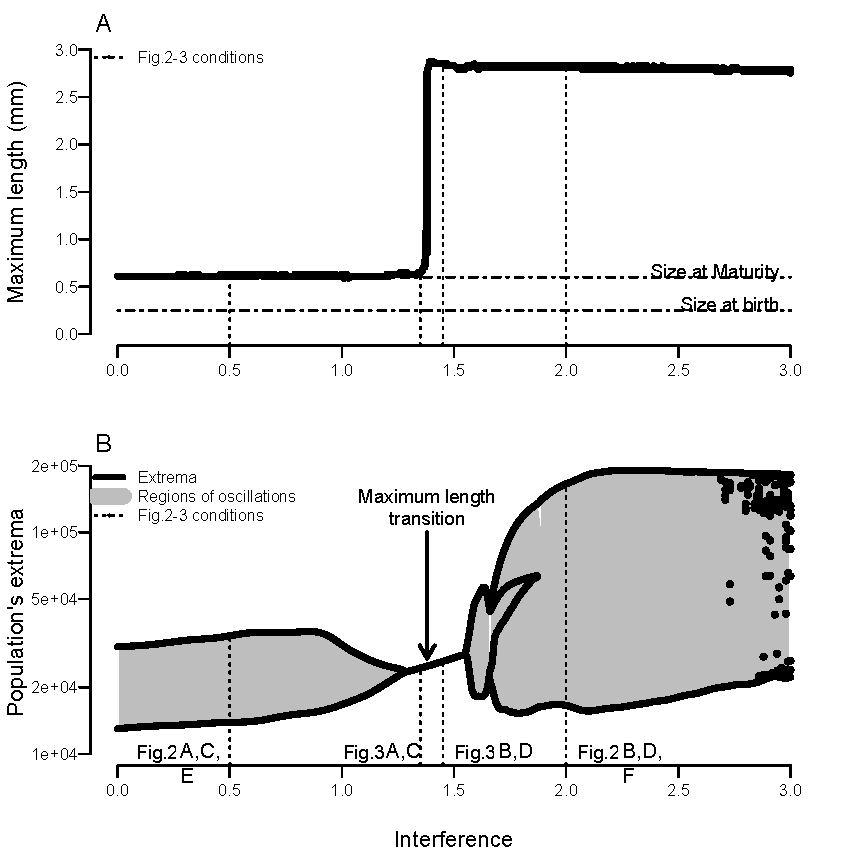
\includegraphics[width=0.85\textwidth]{4_ChapThe1/Fig/Fig1.pdf}
\caption[\lofimage{4_ChapThe1/Fig/Fig1.pdf}Bifurcation over interference]{
Maximum achieved length (A) and total population's extremes (number of
individuals) (B) for increasing values of interference and a low mortality rate
($\mu=0.0065$). Dashed lines mark conditions presented in Figures \ref{Fig4-2}
and \ref{Fig4-3}.
In the bottom plot, thick black lines represent the population's extrema for
each simulation of different values of $I$. The gray areas represent regions
where the population dynamics converges toward a limit cycle. The arrow marks
the transition observed on the top figure.}
\label{Fig4-1}
\end{figure}

Figure \ref{Fig4-1}A shows a very abrupt increase of the maximum length at a
critical value of $I = 1.4$. Below the critical value the maximum achieved
length in the population is just above the length at maturity $l_j=0.6$ mm
($l=0.63$ mm). Above the critical value, the maximum length is close to the
physiologically maximum length $l_m=3$ ($l=2.85$ mm). Interestingly there is no
bi-stability around this critical value.

Figure \ref{Fig4-1}B shows three overall regions of interest: a limit cycle at
low interference, a stable equilibrium at intermediate interference; and a new
limit cycle at high interference. In a small region of interference (around $I =
1.8$) the latter limit cycle has a double period (Sup. Mat. \ref{subsec:SupMat3} and
Figure \ref{Fig4-SM6}) and it becomes irregular at high interference.

\subsection{Juvenile-driven generation cycles}

Without interference ($I=0$), the population converges to a limit cycle that
corresponds to the well-known juvenile-driven generation cycles caused by
exploitative competition \autocites{de-roos1992a,de-roos1997a}. Figure
\ref{Fig4-2} shows a sample dynamics for low interference ($I=0.5$, Figure
\ref{Fig4-2}A,B,C) corresponding to the first dashed line in Figure
\ref{Fig4-1}. Figure \ref{Fig4-2}A presents both the total population dynamics
and the dynamics of its size-structure. These oscillations correspond to
successive waves of cohorts that grow until reaching a reproductive state for a
length $l\geq0.6$ mm. Adults stop growing after reaching maturation, with a
maximum achieved size of $l=0.63$ mm. This is characteristic of juvenile-driven
generation cycles due to exploitative competition
\autocites{de-roos1992a,de-roos2003b}. Figure \ref{Fig4-2}B and C show
respectively the growth rate and the access to the resource as a function of
length. In a purely exploitative competition model, the growth rate is linearly
decreasing with length, and the resource accessibility is constant.
Figure \ref{Fig4-2}B shows that the growth rate is almost linearly decreasing,
although curved upward for $l$ close to $l_j$ ($0.6$ mm), and the access to the
resource is slightly increasing with body size but drops below the minimum
required access $A^*$ (slanting line) for $l > l_j$. The curvature of the growth
rate and the resource accessibility is due to interference competition favoring
bigger individuals.

\begin{figure}[!ht] % Figure 2 
\centering
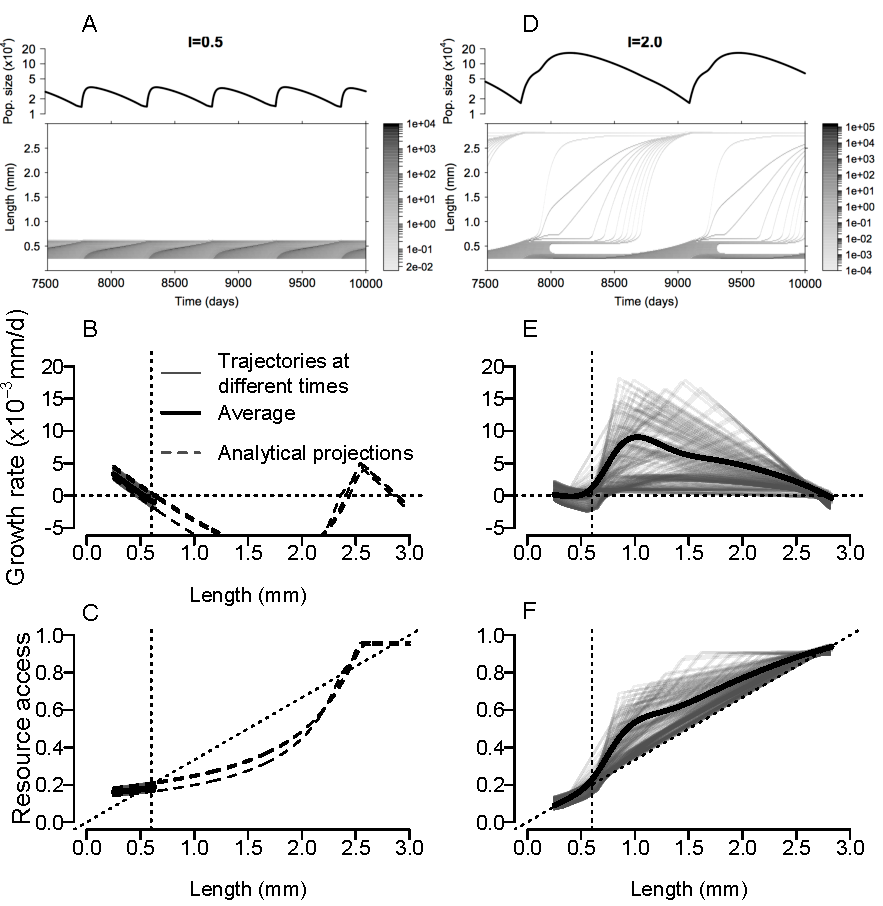
\includegraphics[width=0.85\textwidth]{4_ChapThe1/Fig/Fig2.pdf} 
\caption[\lofimage{4_ChapThe1/Fig/Fig2.pdf}Sample dynamics for $I=0.5$ and
$I=2.0$]{Sample dynamics for $I=0.5$ (A,B,C) and $I=2.0$ (D,E,F). A and D shows the dynamics of
the total population size along with the dynamics of the structure of the
population \autocites{mallard2012a}. B and E represent the growth rates as a
function of length. The vertical dashed line marks the length at maturity, the
horizontal one the $0$ growth rate. Shaded gray lines show phase lines at
different times, and the thick black line is the average growth. C and F show
the resource accessibility as a function of length. The vertical line marks the
length at maturity. The slanting line is the minimum required accessibility
$A^*$. As for B and E, shaded gray lines and thick black lines represent
respectively the different phase lines and the average competition. The dashed
lines represent the analytical projections of $A$ and $g$ over the whole length
range considering the actual state of the population.}
\label{Fig4-2}
\end{figure}

\subsection{Stable equilibrium with small or giant adults}

With intermediate interference the dynamics tend to a stable equilibrium (Figure
\ref{Fig4-1}B). The explanation is that the size-advantage of adult individuals
due to interference reduces the exploitative competition inflicted by the small
ones, thus undoing the mechanism responsible for the juvenile-driven generation
cycles.

The resulting stable equilibrium can be characterized by either a narrow or a
wide population size distribution (Figure \ref{Fig4-3}). For values below the
critical interference level ($I<1.4$, Figure \ref{Fig4-1}A), the curvature of
the growth rate and the resource access functions is insufficient to allow
growth beyond the size at maturation (Figure \ref{Fig4-3}B,C). In this case, an
immigrant of sufficient body size would have a largely positive growth rate and
reach giant sizes, but the individuals born in the population cannot grow into
this size interval.

Beyond the critical interference level ($I>1.4$, Figure \ref{Fig4-3}D,E,F) the
curvature is just strong enough for individuals to experience a secondary
acceleration of their growth rate, eventually reaching giant sizes (Figure
\ref{Fig4-3}D,E). The population size distribution is strongly skewed since the
growth rates stalls around the maturation size. We refer to the minimum of the
growth rate function as the “growth bottleneck”. The rapid increase in growth
rate and resource access beyond the growth bottleneck ($l>0.65$ mm; Figure
\ref{Fig4-3}F) is explained by the increased competitiveness and by the low
density of large individuals. The linear decrease beyond $l=1.3$ mm is due to
the natural shape of the Von Bertalanffy growth function (Sup. Mat.
eq. \eqref{eq:7}).

\begin{figure}[!ht] % Figure 3 
\centering
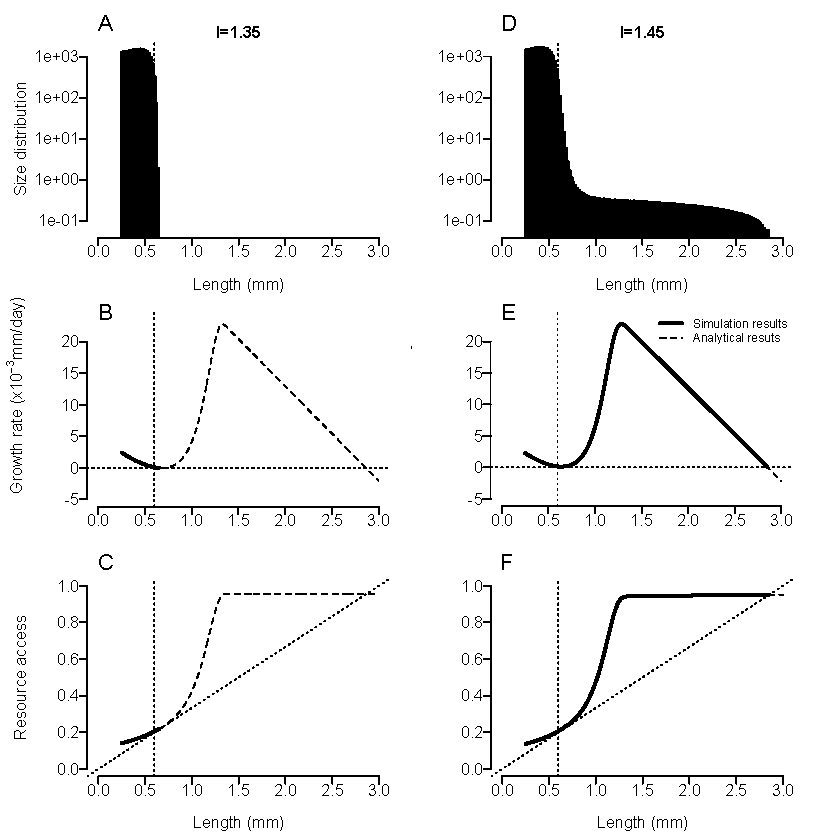
\includegraphics[width=0.85\textwidth]{4_ChapThe1/Fig/Fig3.pdf} 
\caption[\lofimage{4_ChapThe1/Fig/Fig3.pdf}Sample dynamics for $I=1.35$ and
$I=1.45$]{Size distributions (A,D), growth rate (B,E) and accessibility (C,F)
for two conditions of interference producing fixed points, $I=1.35$ (A,B,C) and
$I=1.45$ (D,E,F). The dotted and dashed lines are the same as in Figure
\ref{Fig4-2}.}
\label{Fig4-3}
\end{figure}

Figure \ref{Fig4-1}B shows that beyond $I = 1.56$ interference competition
results in population cycles. Figure \ref{Fig4-2}D, E and F show the details of
a sample run for $I=2.0$. Figure \ref{Fig4-2}D shows that these cycles are
different from the juvenile-driven generation cycles (Figure \ref{Fig4-2}A):
the period of the cycles is almost three times longer and the amplitude is about
$7.5$ times larger. The initial increase in population size corresponds to a
birth pulse due to a cohort of individuals reaching maturity ($l \geq l_j$). At
this moment the population is multi modal and composed of a large number of
immature individuals some newly recruited adults and a few old giant
individuals. This birth pulse is followed by the growth of the recently matured
individuals towards giant body sizes, which decreases the resource accessibility
of the smaller individuals that temporarily stop growing (Figure \ref{Fig4-2}D).
The stalling individuals form two distinct groups: juveniles with $l<0.35$ mm;
and juveniles and adults with $0.5 < l < 0.75$ mm (Figure \ref{Fig4-2}D). During
this period, adults continue to reproduce, increasing the abundance of
juveniles. Due the loss of large individuals, the resource accessibility of
intermediate individuals increases allowing them to progressively grow and reach
giant sizes themselves.
The smallest group remains stalling at small sizes and do not mature. The number
of reproducing individuals slowly decreases due to background mortality, leading
to a decrease in total population size and interference competition. When the
number of adults is low enough, the smaller individuals can start growing again
and reach maturity, leading to a new cycle.

Figure \ref{Fig4-2}E and F show respectively the growth rates and the
accessibility against the length with an interference of $I=2.0$, at different
moments of the cycle (in thin gray lines) and on average (thick black lines).
Individuals with a negative growth rate simply stop growing, and suffer
increased mortality if they are not able to fulfill their maintenance. First, we
see on panel E that the position of the growth bottleneck varies on the x-axis
between $0.33$ and $0.55$ mm, depending on the moment considered in the cycle,
but it always happens at a length smaller than the length at maturity, causing
the accumulation of immature individuals.


The resource accessibility (Figure \ref{Fig4-2}F) shows the same phenomenon,
while accumulating at a size smaller than $l_j$, individuals have an
accessibility below the minimum sustainable value, which explains the negative
growth rate (growth stops and mortality is increased). In the phase of the cycle
where the number of large individuals decreases, the resource accessibility of
the smaller ones increases until becoming sustainable again, and they start
growing again. It is the position of the growth bottleneck below $0.6$ mm that
causes the cycling dynamics.

\subsection{\texorpdfstring{$(I,\mu)$}{(I,mu)} Bifurcation}

The previous examples show the behavior of the model for a relatively low
mortality ($\mu=0.0065$). Yet, mortality is known to have a very important role
in the regulation of the dynamics of structured populations. Figure \ref{Fig4-4}
shows the results of bifurcation runs conducted in the $(I,\mu)$ parameter
space. The upward and downward runs gave identical results suggesting the
absence of bistability.

\begin{figure}[!ht] % Figure 4 
\centering
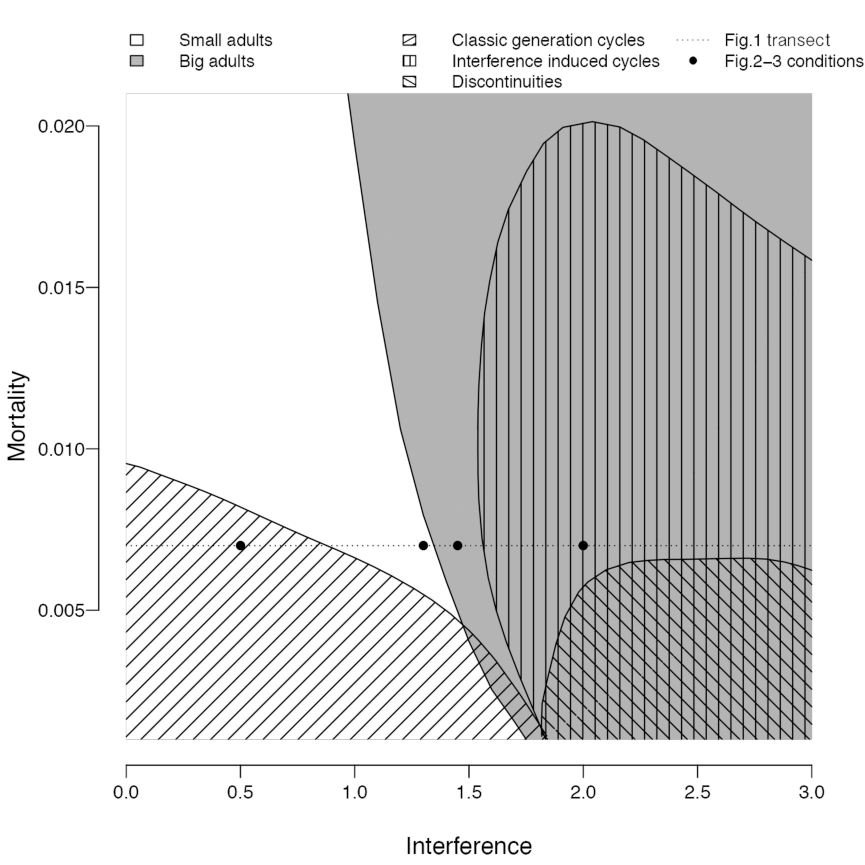
\includegraphics[width=0.85\textwidth]{4_ChapThe1/Fig/Fig4.pdf}
\caption[\lofimage{4_ChapThe1/Fig/Fig4.pdf}$(I,\mu)$ stability
diagram]{Compiled bifurcation diagram in the mortality -- interference
parameter plane. Regions without hatching correspond to regions of stability. White area:
small maximum size. Grey area: giant maximum size. Hatching: type of population
cycle. No bistability was observed. Dashed line: the transect in Figure
\ref{Fig4-1}. Black dots: the locations of the runs in Figure \ref{Fig4-2} and
Figure \ref{Fig4-3}.}
\label{Fig4-4}
\end{figure}

First, Figure \ref{Fig4-4} shows that the parameter space can be separated in
two distinct areas, characterized by either a small ($l=0.63$ mm, white
background) or giant maximum size ($l=2.85$ mm, grey background). The critical
interference level separating these regions is relatively insensitive to the
background mortality ($I \approx 1.2-1.6$).

Second, conform to the theory on exploitative competition
\autocites{de-roos1997a}, increasing background mortality without interference
competition ($I = 0$) tends to stabilize the juvenile-driven generation cycles.
With positive interference competition, the stabilization of these cycles occurs
at a lower mortality rate.
Interference-induced cycles tend to stabilize as well at very high mortality
($>0.02$), but the pattern differs.

At low mortality ($\mu<0.005$) but high interference, the dynamics become
irregular and the size structure exhibits discontinuities. At low mortality and
intermediate interference, between $1.5$ and $2.0$, the situation is more
complex. Indeed, in this region, generation cycles continue to exist although
adults start reaching a length close to $l_m$. But in this region, the
generation cycles are degenerate and some individuals exceptionally manage to
escape the trap of reduced growth rate close to the maturation size and manage
to start growing again, but they are very isolated and the size structure
dynamics is very irregular.

\section{Discussion}

We have shown that interference competition in favor of large individuals is an
interaction that counteracts the consequences of (size-dependent) exploitative
competition. Exploitative competition generally favors small individuals due to
the energetic advantage of a small body size which results from the size scaling
of food intake and maintenance rates
\autocites{peters1986a,persson1998a,de-roos2013a}. This is predicted for most
species by Dynamic Energy Budget theory \autocites{kooijman2000a} and has been
confirmed for the few species for which sufficient empirical data are available
(roach, perch, Daphnia, vendace; De Roos and Persson \citeyear{de-roos2013a}).
Across the gradient of interference competition that we consider (Figure
\ref{Fig4-1}) the overall competitive asymmetry changes gradually from superior
juveniles (due to exploitative competition) to superior adults (due to
interference). In between, the two types of competition more or less balance
each other. Dynamically, this leads to transitions from juvenile-driven
generation cycles to a stable equilibrium to adult-driven generation cycles
(Figure \ref{Fig4-1}).
Interestingly, this pattern is qualitatively similar to the consequences of
varying the size-dependent scaling of exploitative competition in order to give
an energetic advantage to large individuals (without interference competition),
as investigated by \textcite{persson1998a} and \textcite{de-roos2003a}.
The same transitions are found when increasing the slope of the allometric
attack rate function \autocites{persson1998a} or the adult consumption rate
\autocites{de-roos2003a}. The resulting pattern of dynamics is hence similar, but
the underlying mechanisms are different. The parameter values that lead to the
prediction of adult-driven cycles due to exploitative competition are rather
unrealistic for natural populations \autocites{persson1998a,de-roos2003a}. Our
results propose an alternative explanation of adult-driven generation cycles (as
was already speculated by \textcite{de-roos2003a}), which is likely to be more
realistic since it occurs for realistic allometric scaling relations.

Although the interference-induced population cycles (Figure \ref{Fig4-1}, Figure
\ref{Fig4-2}D) are not identical to the adult-driven generation cycles according
to the definition in \textcite{de-roos2003a}, we argue that they should
nevertheless be referred to as “adult-driven” generation cycles. To us, the most
important feature of both types of cycles is the competitive superiority of
large individuals (adults) that prevents a new generation from becoming dominant
until the current adult generation has died out sufficiently. In that sense,
both types of cycles are essentially “adult-driven”. It is useful however, to
distinguish between them in terms of the underlying competition being either
exploitative or interference.

When comparing our results to the effect of size-dependent cannibalism, we
observe two similarities: both interference competition and cannibalism have the
potential to dampen juvenile-driven generation cycles, and both interactions may
lead to the emergence of giant individuals 
\autocites[][this study]{claessen2000a,claessen2002a}. The explanation of the
similarities is that both interactions provide an advantage to large individuals, protecting them from exploitative competition with small individuals.

\subsection{How to detect interference-induced population dynamics empirically?}

The similarity of predictions between interference competition on the one hand,
and cannibalism or exploitative competition on the other hand, implies that when
comparing model predictions with observed data, one needs to be careful in
attributing effects to causes. We need specific criterions that can distinguish
the role of each of these interactions for a given system. For many species this
is rather easy (e.g., we know that roach are not cannibalistic) but may be
difficult in particular for piscivorous fish, which are often candidates for all
three interactions (perch, Arctic char, pike, trout, salmon, cod, etc).
Piscivorous fish have often served as empirical examples for models of
exploitative competition and cannibalism
\autocites{claessen2000a,claessen2002a,persson2003a,de-roos2013a} but the results
may be influenced by interference competition as well.

Before looking into a number of empirical case studies, we will first establish
a list of search images that are indicative of population dynamics caused by
interference competition, based on our model results. The most conspicuous model
prediction is (i) the emergence of giant individuals dominating the resource and
controlling population dynamics. In itself the presence of giants is not
conclusive since it may be due to cannibalism
\autocites{claessen2000a,persson2003a} or exclusive resources for large
individuals. Yet in combination with the following observations it can be taken
as a sign of interference competition. Specifically, (ii) the presence of a
growth bottleneck (Figure \ref{Fig4-3}E) is a sign of interference competition.
In stable equilibrium, these two items together result in (iii) a highly skewed
population size distribution (Figure \ref{Fig4-3}). In cycling populations,
these aspects result in a (iv) bimodal or trimodal size distribution. In both
stable and cycling populations, they result in so-called (v) “double growth
curves”, the result of the secondary growth acceleration caused by interference
competition advantage at large sizes.
Finally, the mechanism driving interference-induced population cycles provides a
telling search image: (vi) for long periods the population is dominated by
large, reproducing adults, whose interference competition deprives juveniles of
resources, resulting in an accumulation of juveniles (and small adults). A new
dominant cohort cannot emerge before the current one has died out sufficiently.
A conspicuous distinction between juvenile-driven generation cycles and
interference-induced generation cycles is hence the typical life history of
individuals. Whereas in the former case individuals grow fast as juveniles and
are quickly outcompeted after reaching maturity, in the latter case individual
growth usually stalls before maturation (the growth bottleneck, Figure
\ref{Fig4-3}E), followed by secondary growth acceleration. (vii) For cases where
population-level data are available but individual-level data are not, a final
search image is the ratio of the average maturation time to the periodicity of
the cycles, used by \textcite{murdoch2002a} to classify
population cycles as either single generation cycles ($ratio = 1$), delayed
feedback cycles ($2\leq ratio \leq 4$) or consumer-resource cycles ($ratio >
6$). For interference-induced cycles, our model shows an average ratio of $1.5$,
whereas our juvenile-driven cycles have a ratio of $0.8$. Generation cycles with
a relatively high ratio could hence be an indication of interference competition.

Using the list (above items i-vi) we re-examine a number of literature case
studies before presenting a more detailed laboratory experiment. 

First, looking at the data used by \textcite{murdoch2002a}, a number of species
display a ratio around the value predicted for interference competition: the
sockeye salmon in Bristol Bay ($ratio=1.2$) and Togiak River ($ratio=1.3$), and
the cod in Iceland \autocite[$ratio=1.6$,]{myers1995a}, the beaver in California
($ratio=1.6$) and Missouri ($ratio=1.4$), and the black bear in Yukon
\autocite[$ratio=1.5$,]{novak1987a}.
These species are known for their territoriality
\autocites{foote1990a,nolet1994a,marshall2010a,sverdrup2011a,ping2011a} and hence
are prone to exhibit interference competition, making it a possible explanation
for the observed cycles.

Second, \textcite{claessen2002a} predict that, for cannibalistic species with a
large gape size such as pike, a likely outcome of population dynamics is a
stable equilibrium with “permanent piscivores”. The authors suggest this as a
possible explanation of the observation of stable populations of Arctic char
with giant individuals permanently present
\autocites{parker1991a,griffiths1994a,hammar2000a}. We argue that these
observations may very well be the result of interference competition. We can
forward two arguments in favor of interference competition: (i) the
cannibalistic explanation requires that the gape width is larger than the one
measured for Arctic char; (ii) the shape of the stable size distribution of the
Arctic char populations are (weakly) bi-modal and hence closer to skewed
distribution based on interference competition (Figure \ref{Fig4-3}D) than the
exponential one based on cannibalism. Arctic char is a territorial species and
hence interference competition is likely to be important in this species. A
closer inspection of empirical case studies should allow us to distinguish
between the alternative hypotheses.

Third, “double growth curves” have been observed in fish populations such as
Arctic char and Eurasian perch \autocites{cren1992a}, and have often been
attributed to cannibalism. Again, these data can be re-interpreted in the
context of interference competition. Even better would be to detect such growth
patterns in non-cannibalistic species (fish or other), but to our knowledge, in
the few empirical studies with sufficient data on individual growth patterns,
this has not been described yet (but see the Collembolan example below).

\subsection{Interference-induced giants in a laboratory experiment}

To our knowledge the only case study providing sufficient data on both the
individual and population levels in order to examine the implications of
size-dependent interference competition is our ongoing laboratory experiments on
small populations of \textit{F. candida}. A full description of the experiment
and analysis is given in Chapter \ref{chap:3-1}, while here we
provide a single time series for the purpose of illustration.

The populations are kept in small boxes (about $5$cm wide) with a plaster
substrate to keep the moisture at its maximum. They are kept in the dark at
constant temperature in incubators and are fed weekly with small pellets
($15\mu$L) of yeast (\textit{Saccharomyces cerevisiae}) dissolved in agar-agar
\autocites{tully2005a,tully2008a}. The food is strongly localized compared to the
surface occupied by the individuals, which creates conditions of high
interference competition. Detailed observation of the foraging behavior confirms
that the larger individuals have almost exclusive access to the resource (Figure
\ref{Fig4-5}).

\begin{figure}[!ht] % Figure 5 
\centering
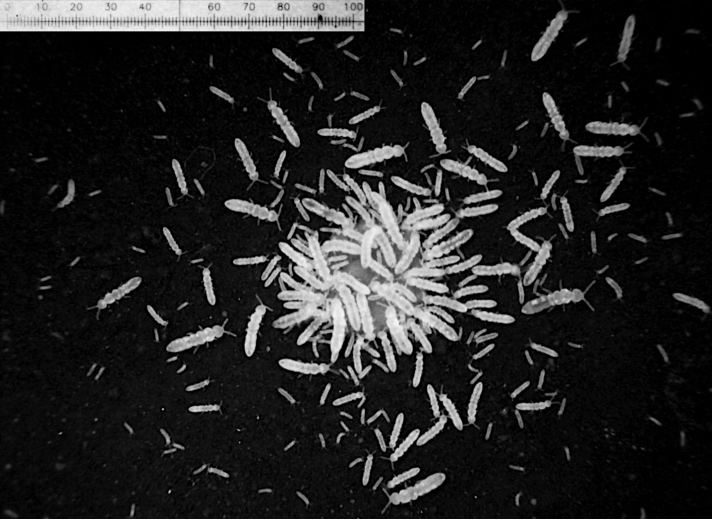
\includegraphics[width=0.85\textwidth]{4_ChapThe1/Fig/Fig5.pdf} 
\caption[\lofimage{4_ChapThe1/Fig/Fig5.pdf}Close up of the resource]{ Close up
of the resource in an experimental population of Collembola Folsomia candida.
The scale corresponds to $10$ mm. The image illustrates interference
competition: the food pellet in the center is dominated by large individuals. }
\label{Fig4-5}
\end{figure}

Using image analysis \autocites{mallard2012a,mallard2013a}, we monitored the
population dynamics and size-structure during more than $800$ days. Figure
\ref{Fig4-6} shows both an empirical population (Figure \ref{Fig4-6}A) and a
model simulation for $I = 1.6$ (Figure \ref{Fig4-6}B), which allows for a close
comparison of model predictions and empirical observations. The comparison
demonstrates two important messages.

First, our model is far from quantitatively accurate. In terms of both absolute
and relative numbers the model is clearly incorrect. Second, our models provides
an interesting qualitative description of the population cycles and hence a
plausible explanation of the observed population dynamics. Specifically, the
“search image” description of the cycles (see item (vi) of the list above) is a
good description of the empirical observations. Giant individuals dominate the
population for extended periods, whereas juveniles accumulate close to the
maturation size. A new dominant cohort is predicted to emerge only when the
giant size class has sufficiently reduced in number. To test this prediction, we
plotted the number of giants and the number of recruiting adults (\textit{i.e.},
a growing cohort in the lower panels). The model predicts that the intermediates
peak when the giants are lowest. The empirical data confirm this pattern, albeit
more noisily, for the second, third, fourth and sixth cohorts. Also, the
predicted and observed patterns of size-structure dynamics (lower panels) are
strikingly similar. A third message from the empirical data is that this cannot
be interpreted as juvenile-driven generation cycles. Adults reach sizes well
beyond the maturation size and the demise of adults predates the emergence of
the next dominant cohort. Both observations are in contradiction to the
description of juvenile-driven generation cycles.

The choice of the example simulation we plotted in Figure \ref{Fig4-6}B was
motivated by the observation that a minority of the experimental populations exhibit
population cycles; the rest appear to be close to an equilibrium state. We
interpret this observation as indicative that the system is close to a
bifurcation point; hence the value of $I = 1.6$.

We argue that the observed dynamics of \textit{F. candida} provide qualitative
(but not quantitative) support for the underlying mechanisms of
interference-induced population cycles.

\begin{figure}[!ht] % Figure 6 
\centering
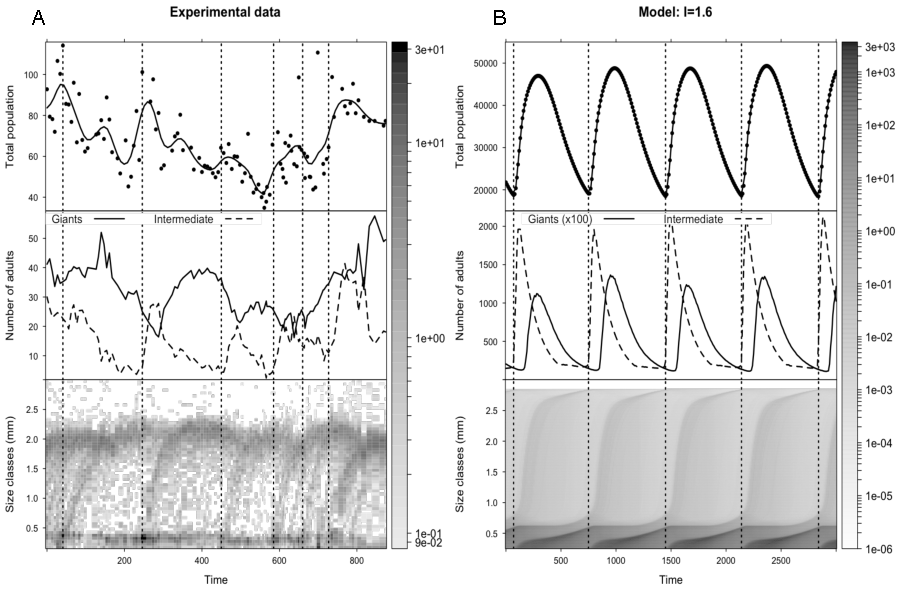
\includegraphics[width=0.95\textwidth]{4_ChapThe1/Fig/Fig6.pdf} 
\caption[\lofimage{4_ChapThe1/Fig/Fig6.pdf}Experiment -- model comparison]{Total
population dynamics (top panels), dynamics of giants and intermediate adults
(middle panels) and dynamics of the size structure (bottom panel) for (A) an
experimental population of \textit{F. candida} bred with weekly resource input
and (B) a model simulation with interference set at $I=1.6$. The vertical
dashed lines mark each cohort cycle. }
\label{Fig4-6}
\end{figure}

\subsection{Sensitivity to energy allocation rules }

An important question is whether our results are the consequence of the specific
energy budget model that we have chosen for our model. Our model uses the
kappa-rule, which assumes that a fixed proportion ($\kappa$) of the energy
budget is allocated to maintenance plus growth while the remainder ($1-\kappa$)
goes to reproduction (see Sup. Mat. \ref{subsubsec:SupMat21}). This implies
that when the energy intake goes down, energy will be rechanneled from growth to maintenance, until growth
eventually stops while reproduction still goes on. For even lower energy intake,
energy will be rechanneled from reproduction to maintenance. This implies that
individuals continue reproducing after reaching their maximum size – a scenario
that is realistic for a wide range of species including Collembolans.

In order to test the robustness of our results to this fundamental assumption,
we have developed an alternative model with a contrasting energy allocation
rule. A rule that is often used to model fish growth is the so-called
net-production model: the energy intake rate is first used to cover maintenance,
and the surplus energy is split between growth and reproduction using a constant
proportion. This rule implies that individuals reaching their maximum size stop
reproducing.

Our alternative model based on net-production allocation gives qualitatively the
same results as the one based on the kappa rule (Sup. Mat. \ref{subsec:SupMat4}). This
shows that our model predictions do not depend on the specific energy allocation rule.

\section*{Concluding remarks}

Our objective was to investigate the consequences of size-dependent interference
competition on population dynamics, complementing the existing results on
size-dependent exploitative competition and cannibalism. For this purpose we
designed a simple, size-structured model that captures what we believe to be the
essential aspects of size-dependent interference competition. The model is hence
not designed to specifically predict the population dynamics of any particular
species, although we have chosen to parameterize the model as much as possible
to our laboratory species F. candida. The model analysis has demonstrated that
interference has interesting dynamical consequences, some of which are akin to
consequences of other interactions. Our analysis of previous and new empirical
data has shown that there is a potential for the detection of these dynamics in
laboratory and natural populations.

\section*{Acknowledgement} 
This research was supported by a French grant from
the French National Research Agency (ANR EvoRange), reference ANR-09-PEXT-011.
The funders had no role in study design, data collection and analysis, decision
to publish, or preparation of the manuscript.

\newpage
\section{Supplementary materials}\label{sec:SupMat}
\subsection{Experimental support for PSP assumptions}\label{subsec:SupMat1}

The KM-model relies on basic assumptions regarding resource allocation that can
be verified on experimental data collected on isolated individuals of our model
species, the Collembola \textit{Folsomia candida}.

\subsubsection{Methods}

The collembolans are maintained in the laboratory in polyethylene vials
(diameter $52$mm, height $65$mm) filled with a $30$mm width layer of a plaster
of Paris mixed with china ink to facilitate detection of the individuals. Food
is provided by offering small dried pellets of a mixture of agar and dried yeast
in standardized concentration and volume \autocites{tully2008a}.
The rearing boxes where kept in incubators at $21 \pm 0.5\degres$C and the
plaster humidified to maintain a constant humidity within the boxes ($\approx
100\%$ RH). We followed $220$ isolated individuals and regularly measured their
body size (using digital pictures) and fecundity (the size of the layed
clutches).

\subsubsection{Growth trajectories and dependence on resources}

The model supposes that for a constant food level the body length follows a Von
Bertalanffy growth curve, and that the maximum size and the growth rate both
depend on food level. These three aspects are valid for our experimental species
as shown by Figure \ref{Fig4-SM1}.

\begin{figure}[!ht] % Figure 6 
\centering
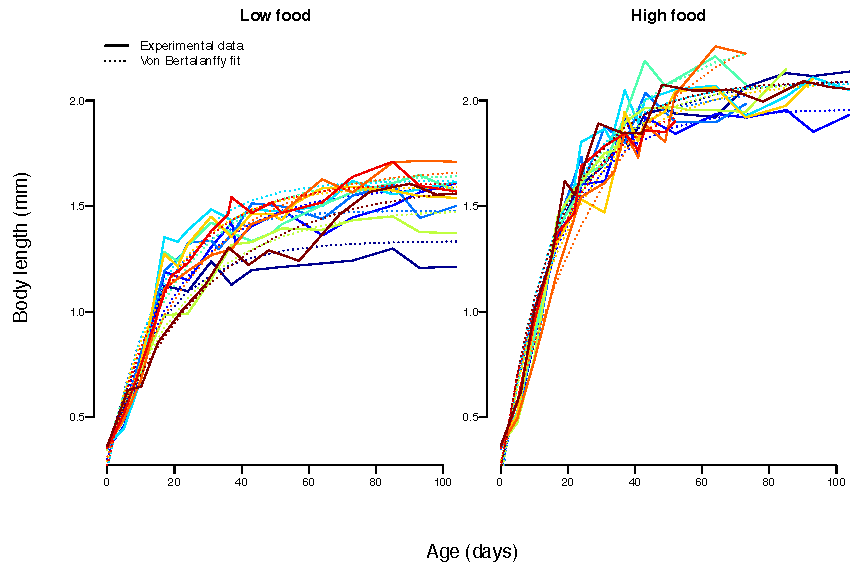
\includegraphics[width=0.85\textwidth]{4_ChapThe1/Fig/FigSM1.pdf} 
\caption[\lofimage{4_ChapThe1/Fig/FigSM1.pdf}Experimental growth
trajectories]{Growth
trajectories (plain lines) and corresponding von Bertalanffy fit  (dotted lines) in two different resource conditions.}
\label{Fig4-SM1}
\end{figure}

\subsubsection{Reproduction}

Furthermore, the KM-model predicts that reproduction increases with the food
level and scales with the square of body length. Figure \ref{Fig4-SM2} shows
that both relations are valid for \textit{F. candida}.

\begin{figure}[!ht] % Figure 6 
\centering
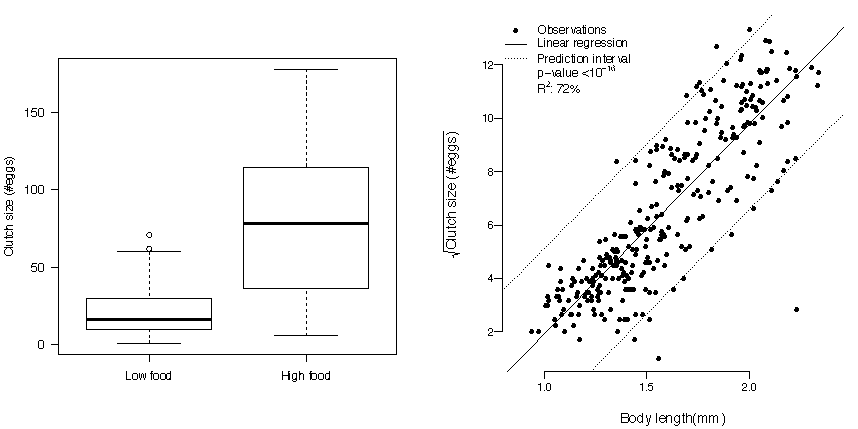
\includegraphics[width=0.85\textwidth]{4_ChapThe1/Fig/FigSM2.pdf}
\caption[\lofimage{4_ChapThe1/Fig/FigSM2.pdf}Experimental measure
of reproduction]{Reproduction (clutch size) in two different resource
conditions, and square root of clutch size against body length. Regression statistics for the latter are extremely significant.}
\label{Fig4-SM2}
\end{figure}

\subsubsection{Size at Birth}

The model assumes that size at birth is independent from food availability.
Figure \ref{Fig4-SM3} shows the egg diameter as a measure correlated to the body
length at birth in two different resource conditions. Although the difference is
significant due to very large sample sizes, the difference between the two means
is quite low and we can consider that the assumption that length at birth is
constant over food availability is valid for our model species.

\begin{figure}[!ht] % Figure 6 
\centering
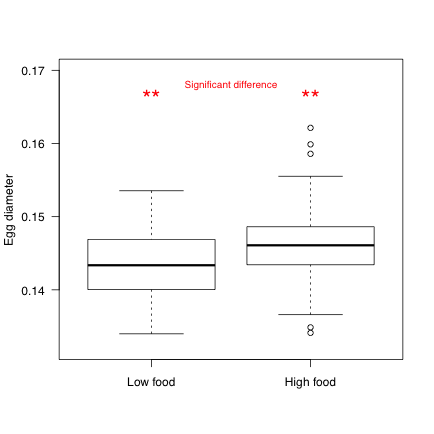
\includegraphics[width=0.7\textwidth]{4_ChapThe1/Fig/FigSM3.pdf}
\caption[\lofimage{4_ChapThe1/Fig/FigSM3.pdf}Experimental measure of size
at birth]{Egg diameter as a proxy for size at birth in two different resource
conditions.}
\label{Fig4-SM3}
\end{figure}

\subsubsection{Maturation length}

Finally, the KM-model assums a length at maturity constant over food
availability and population density. In experimental populations, it is
impossible to assess the body length at maturation. We then realized measures of
size on isolated individuals. This gave us access to the body length at the
first clutch in two different resource conditions, wich is longer than the
length at maturity but the closest proxy available in our experimental
conditions. Figure \ref{Fig4-SM4} shows that the model assumption concerning
length at maturity is not supported by our experimental population. Nevertheless, we
consider that this assumption is not a primary assumption, and considering the
length at maturity constant in the model simplify it without changing
dramatically its behavior.

\begin{figure}[!ht] % Figure 6 
\centering
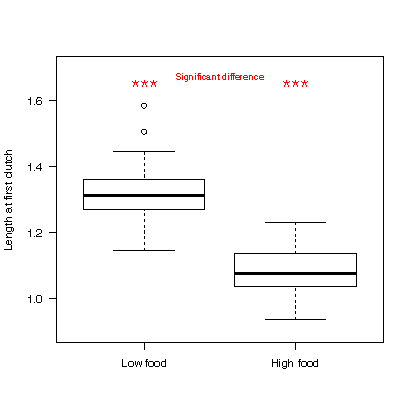
\includegraphics[width=0.7\textwidth]{4_ChapThe1/Fig/FigSM4.pdf}
\caption[\lofimage{4_ChapThe1/Fig/FigSM4.pdf}Experimental measure of
length at maturity]{Length at first clutch in two different resource
conditions.}
\label{Fig4-SM4}
\end{figure}

\subsection{Individual level model}\label{subsec:SupMat2}

Individual interactions being defined as previously described, the individual
rates depend directly on a dynamic energy budget chosen. The choice we made is
based on the $\kappa$-rule \autocite[][Figure
\ref{Fig4-SM5}]{kooijman1984a,de-roos1997a}, which assumes that a fixed
proportion ($\kappa$) of the energy intake (thick black arrow in Figure
\ref{Fig4-SM5}) is allocated to maintenance plus growth while the remainder
($1-\kappa$) goes to reproduction. This implies that when the energy intake goes
down, energy will be rechanneled from growth to maintenance, until growth eventually stops while
reproduction still goes on (dotted arrow in Figure \ref{Fig4-SM5}). For even lower energy
intake, energy will be rechanneled from reproduction to maintenance. This rule
implies that individuals continue reproducing after reaching their maximum size
-- a scenario that is realistic for a wide range of species including
Collembolans. When the energy intake is insufficient to cover maintenance, the
individual is assumed to die.

To be general, let's call $F$ the functionnal response to the resource and $l$
the individual length. In our model, $F$ is the access to the resource
$A(t,l)$.
The energy intake $E_{in}$ of an individual is a function of the functionnal
response and the individual length:
\[ E_{in}=\epsilon\cdot F\cdot l^{2} \]

where $\epsilon$ is a conversion coefficient. And the metabolism
is 
\[
\rho\cdot l^{3}
\]
 where $\rho$ is a parameter. 

\subsubsection*{$\kappa$-rule}\label{subsubsec:SupMat21}


In the $\kappa$-rule, the energy intake (thick black arrow) is first
divided into $1-\kappa$ allocated to reproduction and $\kappa$ allocated
to metabolism, and if all the metabolism cost is paid, the rest of
this $\kappa$ fraction goes to growth (Figure \ref{Fig4-SM5}). 

\begin{figure}[ht] % Figure 6 
\centering
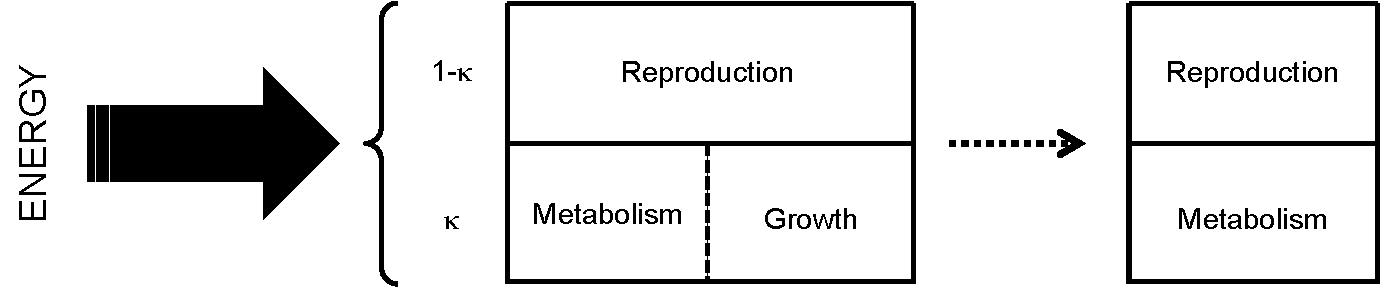
\includegraphics[width=0.95\textwidth]{4_ChapThe1/Fig/KRule}
\caption[\lofimage{4_ChapThe1/Fig/KRule}Details of the
$\kappa$-rule]{Description of the $\kappa$-rule and its implications}
\label{Fig4-SM5}
\end{figure}

Once the individual has reached
it's maximum size (dashed arrow), the energy intake is allocated to
the metabolism and the rest to reproduction. We not that even after
reaching its maximum size, an individual continues to reproduce until
it cannot fulfill its metabolism anymore and dies.

Given the rules of energy allocation, we can write the individual
growth rate and reproduction rate as functions of the functional response
and the individual length.

Birth rate represents the production of newborns (mass or weight $w$)
from the energy absorbed, and can be written:
\begin{eqnarray*}
b_{\kappa}(l) & = & (1-\kappa)\cdot\epsilon\cdot Fl^{2}\\
 & = & r_{m}\cdot Fl^{2}
\end{eqnarray*}


where $r_{m}=(1-\kappa)\cdot\epsilon$ is a reproduction rate. We
note that the birth rate increases with body length following a parabola. 

As opposed to reproduction which is an increase in weight, growth
is the increase in body length $l$. We then define the parameter
$c$ as a length to weight coefficient such as $w=c\cdot l^{3}$,
which leads to 
\[
\frac{dw}{dl}=3c\cdot l^{2}\Leftrightarrow\frac{dl}{dw}=\frac{1}{3cl^{2}}
\]


Expressed in words, growth rate is the fraction $\kappa$ of the energy
intake minus the cost of metabolism. That is to say:

\[
g_{\kappa}(l)=\frac{dl}{dt}=\frac{dw}{dt}\cdot\frac{dl}{dw}=\frac{1}{3cl^{2}}\cdot\frac{dw}{dt}
\]


where $\frac{dw}{dt}$, the change in weight over time is 
\[
\frac{dw}{dt}=\kappa\cdot\epsilon\cdot Fl^{2}-\rho l^{3}
\]
The growth rate in body length is then 
\begin{eqnarray*}
g_{\kappa} & = & \frac{1}{3cl^{2}}\cdot\left(\kappa\cdot\epsilon\cdot Fl^{2}-\rho l^{3}\right)\\
 & = & \frac{1}{3c}\cdot\left(\kappa\cdot\epsilon\cdot F-\rho l\right)\\
 & = & \frac{\rho}{3c}\cdot\left(\frac{\kappa\epsilon}{\rho}F-l\right)
\end{eqnarray*}
Let's define ${\displaystyle \gamma=\frac{\rho}{3c}}$ and ${\displaystyle
l_{m}=\frac{\kappa\epsilon}{\rho}}$, respectively the von Bertalanffy growth
parameter and the absolute maximum length, that is to say the length at infinite resources and
without competition, we can then write the growth rate in the case
of the $\kappa$-rule as follows:

\begin{equation}
g_{\kappa}(l)=\gamma\cdot\left(l_m\cdot F-l\right)
\label{eq:7}
\end{equation}


which integrates as the von Bertalanffy growth function for an isolated
individual. We can see that with the biological interpretations of
$\gamma$ and $l_m$, we don't need to have access to the value
of $\kappa$ to parametrize the model.

\subsubsection{Population level integration}

At the population level, the number of individuals at time t is given by the
integral
\begin{equation}
\label{eq_10}
\int_{l_b}^{l_m}\!n(t,l)\,\mathrm{d}l
\end{equation}
where $n(t,l)$ is the number of individuals of length $l$ at time $t$. The
population dynamics is the described by the following partial differential
equation and limit conditions \autocites{kooijman1984a,de-roos1997a}
\begin{align}
\label{eq_11}
\frac{\partial n(t,l)}{\partial t}+\frac{\partial g(t,l) \cdot n(t,l)}{\partial l}=-\mu \cdot n(t,l) \\
g(t,l_b) \cdot n(t,l_b)= \int_{l_b} ^{l_m} \! b(t,l)\cdot n(t,l)\, \mathrm(d)l
\end{align}
and the initial condition for the population $n(0,l)=\Psi(l)$ where $\Psi(l)$ is
a chosen size distribution. As the $i$-state determines the sate of an
individual, the state of the population, or $p$-state, characterizes the
composition of the structured population modeled, using a density function over
the $i$-states space. 

\newpage
\subsection{Dynamics for I=1.6 and I=1.7}\label{subsec:SupMat3}

\begin{figure}[H] % Figure 6 
\centering
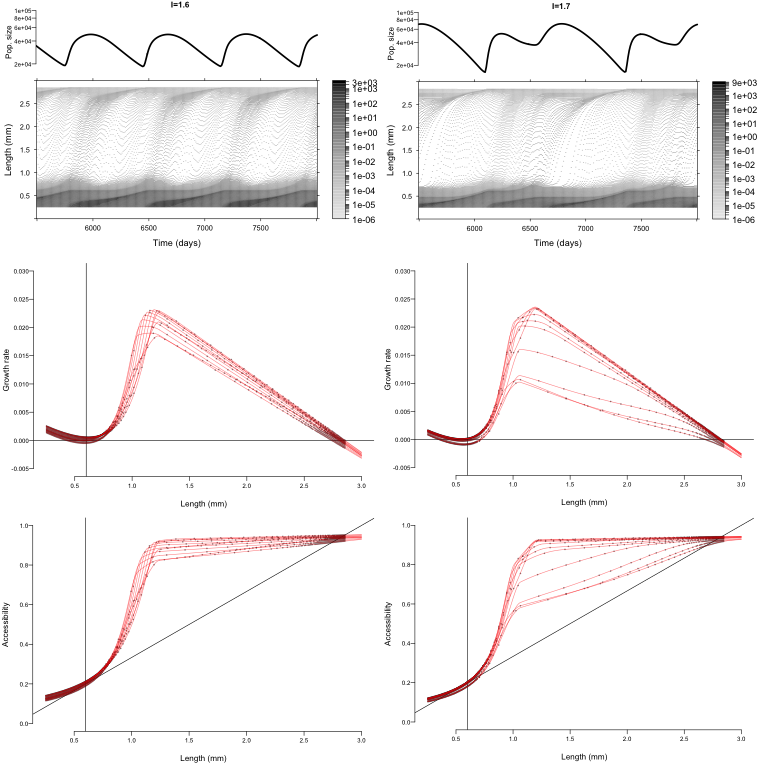
\includegraphics[width=0.95\textwidth]{4_ChapThe1/Fig/FigSM6}
\caption[\lofimage{4_ChapThe1/Fig/FigSM6}Sample dynamics for I=1.6 and
I=1.7]{Population dynamics, growth rate and access to the resource for interference values of $1.6$ and $1.7$. The red lines are the analytical calculations given the state of the population.}
\label{Fig4-SM6}
\end{figure}

\subsection{An alternative energy allocation rule: the net production
model}\label{subsec:SupMat4}

\subsubsection{Description of the Net Production Model}

The $\kappa$-rule is not the only energy allocation rule described in the
literature, although it is one of the most used. Another commonly used rule is the net
production model (Figure \ref{Fig4-SM7}).

\begin{figure}[!ht] % Figure 6 
\centering
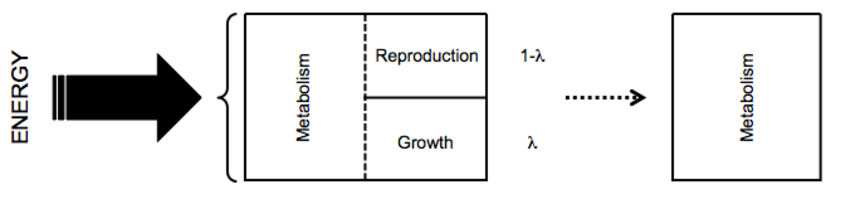
\includegraphics[width=0.95\textwidth]{4_ChapThe1/Fig/FigSM7}
\caption[\lofimage{4_ChapThe1/Fig/FigSM7}Details of the Net
Production model]{Description of the net production model and its implications}
\label{Fig4-SM7}
\end{figure}

In the net production model, the energy intake is first allocated to metabolism.
If some energy is left after fulfilling metabolism, the energy is divided
between growth (fraction $\lambda$) and reproduction (fraction $1-\lambda$).
Once the individual stops growing, meaning it can only fulfill its metabolism, it stops
reproducing at the same time. This is the fundamental difference between the two
rules.

Given the assumptions concerning energy intake and metabolism, we can write the
individual growth rate and reproduction rate as functions of the functional
response and the individual length.

As before, the growth rate in body length can be written as follows:
\[
g_{\text{NP}}=\frac{1}{3cl^{2}}\cdot\frac{dw}{dt}
\]


where $\frac{dw}{dt}$, the change in wheight over time is a fraction
$\lambda$ of what is left after paying for the metabolism: 
\[
\frac{dw}{dt}=\lambda\cdot\left(\epsilon\cdot Fl^{2}-\rho l^{3}\right)
\]


We can hence write the growth rate as follows:
\begin{eqnarray*}
g_{\text{NP}} & = & \frac{1}{3cl^{2}}\cdot\lambda\cdot\left(\epsilon\cdot Fl^{2}-\rho l^{3}\right)\\
 & = & \lambda\cdot\frac{1}{3c}\cdot\left(\epsilon\cdot F-\rho l\right)\\
 & = & \lambda\cdot\frac{\rho}{3c}\cdot\left(\frac{\epsilon}{\rho}F-l\right)
\end{eqnarray*}


Using ${\displaystyle \xi=\lambda\frac{\rho}{3c}}$ and ${\displaystyle L_{NP}=\frac{\epsilon}{\rho}}$
as the von Bertalanffy growth parameter and the absolute maximum length,
we can write the growth rate as:
\[
g_{\text{NP}}(l)=\xi\cdot\left(L_{NP}\cdot F-l\right)
\]


We see that $g_{\kappa}$ and $g_{\text{NP}}$ have the exact same
form. Although the definition of the parameters differ, their biological
interpretation remain the same, with respectively $\gamma$ and $\xi$
the von Bertalanffy growth parameters and $l_m$ and $L_{NP}$ the
absolute maximum length. 

As previously, the birth rate is the increase in mass of newborns:
\[
b_{\text{NP}}(l)=\frac{dw}{dt}\cdot\frac{1}{\omega}
\]
where $\omega$ is the weight of on newborn. With the net production
model, the birth rate is the fraction $1-\lambda$ of the energy left
after fulfilling metabolism:
\begin{eqnarray*}
b_{\text{NP}}(l) & = & \frac{1}{\omega}\cdot(1-\lambda)\cdot\left(\epsilon\cdot Fl^{2}-\rho l^{3}\right)\\
 & = & \frac{1}{\omega}\cdot(1-\lambda)\cdot\rho l^{2}\cdot\left(\frac{\epsilon}{\rho}\cdot F-l\right)
\end{eqnarray*}


Multiplying by $\frac{\lambda}{\lambda}$ we can identify the growth
function $g_{\text{NP}}$:

\begin{eqnarray*}
b_{\text{NP}}(l) & = & \frac{3c}{\omega}\cdot(1-\lambda)\cdot\underbrace{\frac{\lambda}{\lambda}\cdot\frac{\rho}{3c}\cdot\left(\frac{\epsilon}{\rho}\cdot F-l\right)}\cdot l^{2}\\
 & = & \frac{3c}{\omega}\cdot\frac{(1-\lambda)}{\lambda}\cdot\qquad\quad g_{\text{NP}}(l)\;\qquad\cdot l^{2}
\end{eqnarray*}


Furthermore, with $w=3c\cdot l^{3}$, we can write $\omega=c\cdot l_b^{3}$
where $l_b$ is the body length at birth. We then have:
\begin{eqnarray*}
b_{\text{NP}}(l) & = & \frac{(1-\lambda)}{\lambda}\cdot\frac{3}{l_b^{3}}\cdot g_{\text{NP}}(l)\cdot l^{2}
\end{eqnarray*}


We define the parameter ${\displaystyle \beta=\frac{(1-\lambda)}{\lambda}\cdot\frac{3}{l_b^{3}}}$,
and the birth rate writes as
\[
b_{\text{NP}}(l)=\beta\cdot g_{\text{NP}}(l)\cdot l^{2}
\]


We can see that this time that the birth rate is a third degree polynom
which first increases with $l$, and then decreases to $0$ when the
individuals stops growing at $l=l_m\cdot F$.

\subsubsection{From one rule to the other}

In our model, we used the $\kappa$-rule with parameters $\gamma$ and $L_m$
estimated using data from experiments on the collembolan \textit{Folsomia
candida}.
The parameter $L_b$ is also estimated using the same experiments. To convert the
model to a net production energy allocation rule, we can keep the same equation for
the growth function with the same parameters, and simply choose the parameter
$\beta$, knowing the length at birth $L_b$, so that the model behaves similarly
to the $\kappa$-rule model in absence of interference competition and then look at the
effect of interference in the net production model case.

\subsubsection{Bifurcation over interference}

We fixed the value of $\beta$ at $1000$. We then used the same protocol as
described in the methods to investigate the impact of the level of interference on the
dynamics of a structured population in the case of the net production model.

\begin{figure}[!ht] % Figure 6 
\centering
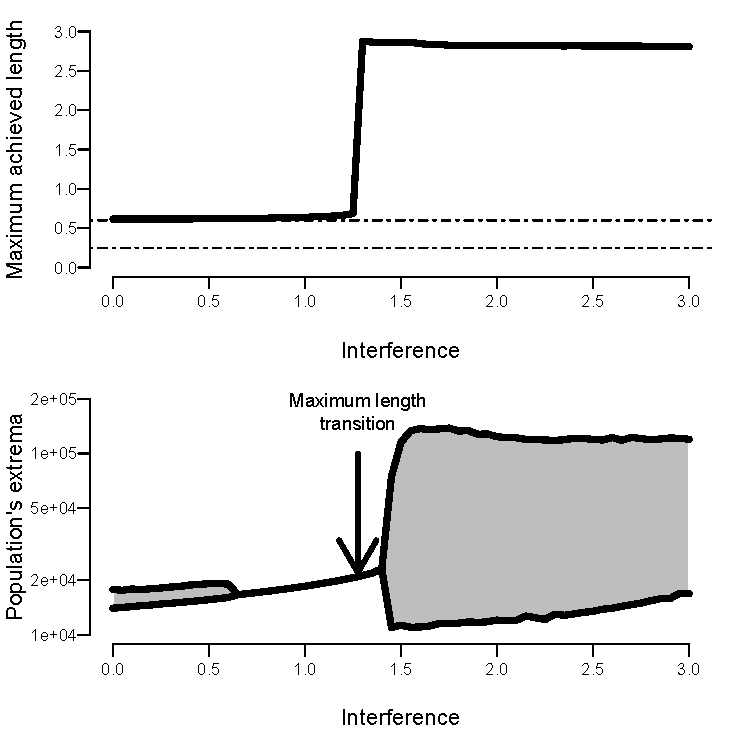
\includegraphics[width=0.95\textwidth]{4_ChapThe1/Fig/FigSM8}
\caption[\lofimage{4_ChapThe1/Fig/FigSM8}Bifurcation over interference
(net production model)]{Maximum achieved length and total population's extremes
for increasing values of interference and a low mortality rate ($\mu=0.0065$).}
\label{Fig4-SM8}
\end{figure}

Figure \ref{Fig4-SM8} shows that the qualitative behavior of the model is the
same as described previously. Indeed, we observe that an increased value of interference
first has a stabilizing effect on the cycles that were present with pure
exploitation.

Furthermore, as previously described, the maximum achieved length in the
population first stays very close to the maturation length but the brutally
reaches a length close to the maximum possible length at infinite resources.
This transition happens in a period where the population structure is stable.

Finally, a higher value of interference destabilizes the structure to limit
cycles with very high amplitude compared to the generation cycles at low
interference. The period of these cycles is also greatly increased, and the
characteristics of the cycles correspond to the “interference-induced cycles”
described for the $\kappa$-rule version of the model.

\subsubsection{Sample simulations}

Looking at sample simulation (Figure \ref{Fig4-SM9} and Figure \ref{Fig4-SM10}),
we can see that although the exact shape of the cycles may differ from the
$\kappa$-rule version, the qualitative dynamics observed for different key
values of interference show the same patterns as previously described. The following figures detail the
population dynamics, the dynamics of the structure, the growth rate as a
function of body length, the access to the resource as a function of body
length, and the birth rate as a function of body length. The birth rate is added
to illustrate the decrease to $0$ when the body growth rate reaches $0$.

\begin{figure}[!ht] % Figure 6 
\centering
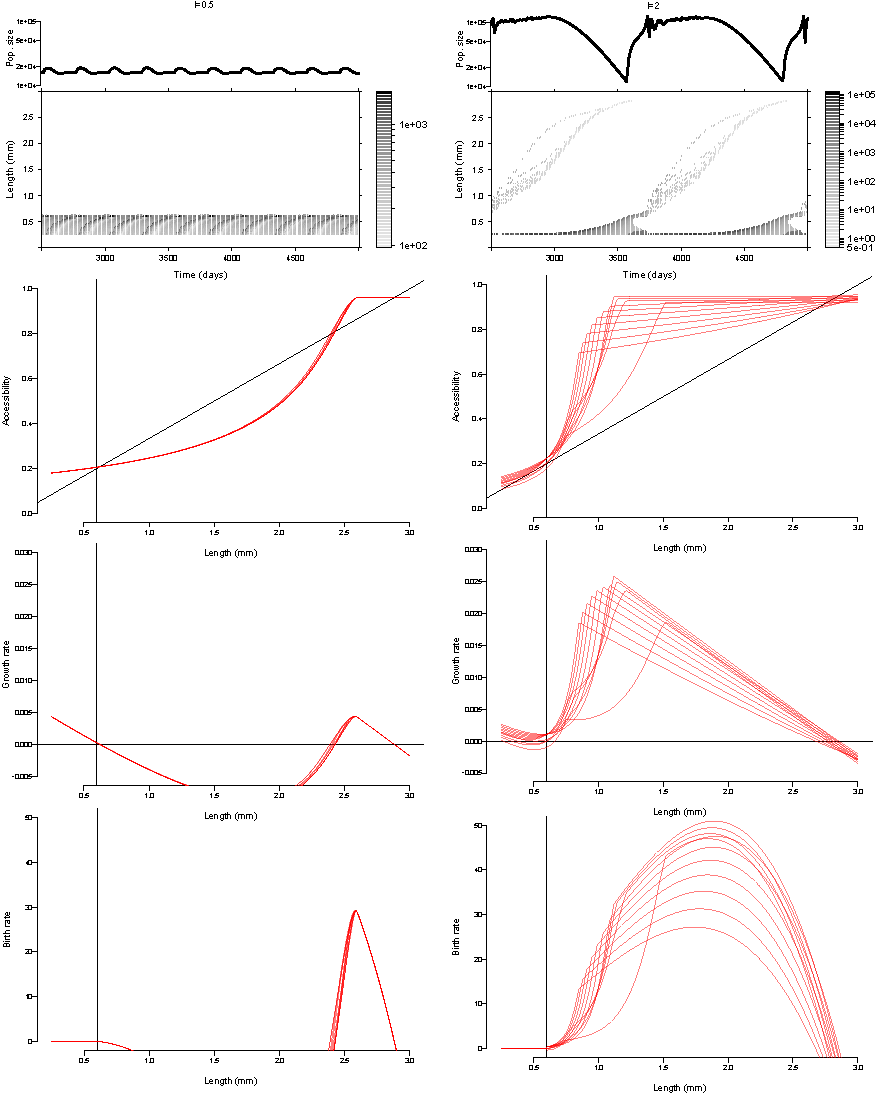
\includegraphics[width=0.95\textwidth]{4_ChapThe1/Fig/FigSM9}
\caption[\lofimage{4_ChapThe1/Fig/FigSM9}Sample simulation for I=0.5
and I=2.0 (net production model)]{Population dynamics, access to the resource,
growth rate and reproduction rate for interference values of $0.5$ and $2.0$. The red lines are the analytical calculations given the state of the population.}
\label{Fig4-SM9}
\end{figure}

\begin{figure}[!ht] % Figure 6 
\centering
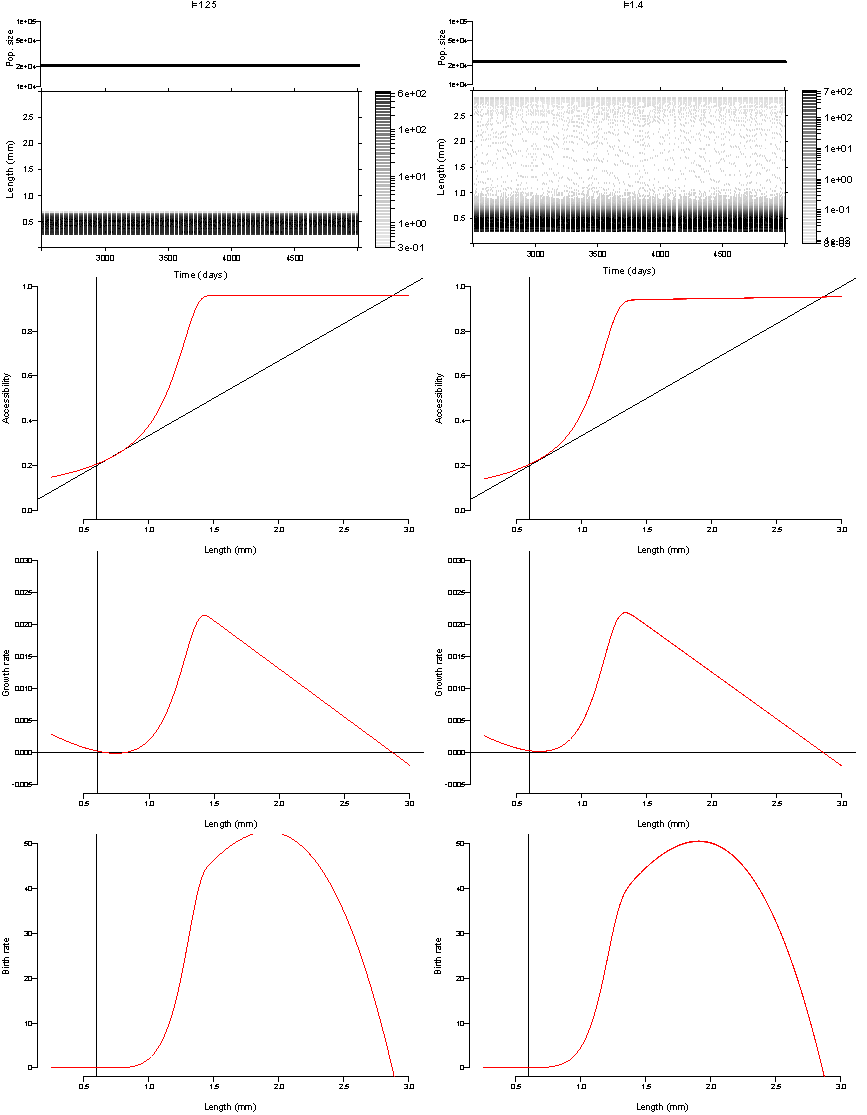
\includegraphics[width=0.95\textwidth]{4_ChapThe1/Fig/FigSM10}
\caption[\lofimage{4_ChapThe1/Fig/FigSM10}Sample simulation for I=1.25
and I=1.45 (net production model)]{Population dynamics, access to the resource,
growth rate and reproduction rate for interference values of $1.25$ and $1.4$. The red lines are
the analytical calculations given the state of the population.}
\label{Fig4-SM10}
\end{figure}

\subsubsection{Discussion}

This study of the model with the net production energy budget implemented showed
that the important results obtained with the $\kappa$-rule version of the model
are still valid under the assumptions of the net production model. This was expected
considering that the dynamics produced by the model with interference are caused
by the progressive superiority acquired by adults while growing when
interference is high. In a population with giant individuals and high
interference, it is the presence of these adults that regulates the population
dynamics rather than the production of young individuals that will compete with
them.

Hence, even though the net production model relies on a very different
assumption concerning reproduction, especially for large individuals, as shown
by Figure \ref{Fig4-SM11} where the birth rate is computed in a case with
infinite resources and no interference, when interference is present, the regulation of
the dynamics shifts from dominated by the juveniles to dominated by the adults,
and the differences between the two energetic rules do not matter in driving the
qualitative dynamics.

\begin{figure}[!ht] % Figure 6 
\centering
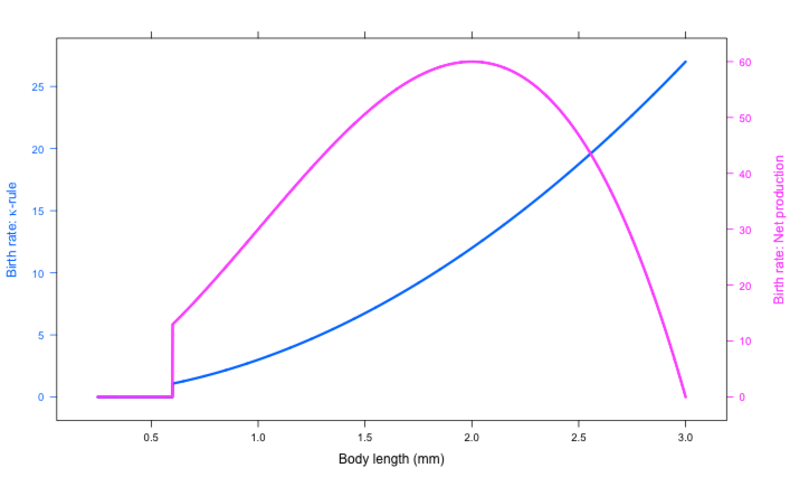
\includegraphics[width=0.95\textwidth]{4_ChapThe1/Fig/FigSM11}
\caption[\lofimage{4_ChapThe1/Fig/FigSM11}Theoretical birth rate for the $\kappa$-rule and the net production model with
$0$ interference]{
Theoretical birth rate for the $\kappa$-rule and the net production model with
$0$ interference.}
\label{Fig4-SM11}
\end{figure}

\subsection{Graphical illustration of competitive superiority of length
\texorpdfstring{$l_{\beta}$}{l_beta} over length
\texorpdfstring{$l_{\alpha}$}{l_alpha}}\label{subsec:SupMat5}

\begin{figure}[!ht] % Figure 6 
\centering
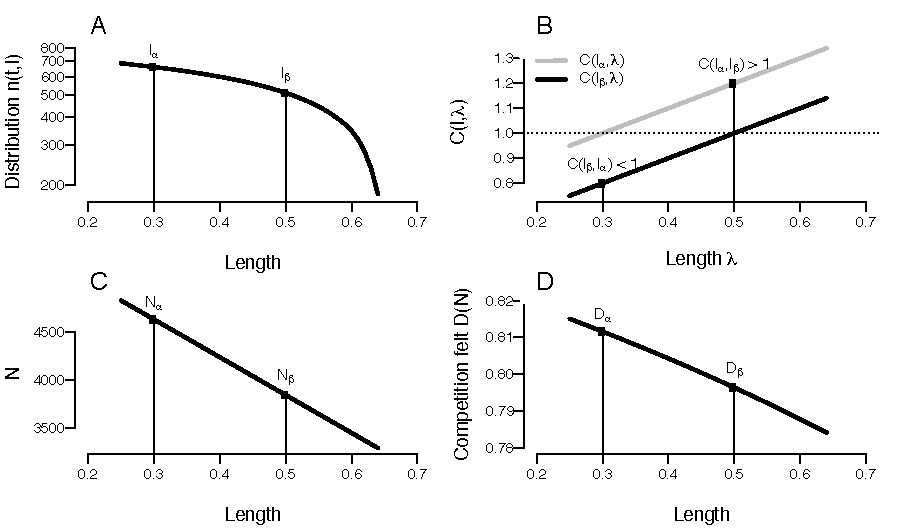
\includegraphics[width=0.95\textwidth]{4_ChapThe1/Fig/FigSM12} 
\caption[\lofimage{4_ChapThe1/Fig/FigSM12}Graphical illustration of competitive superiority of $l_{\beta}$ over
$l_{\alpha}$ when $l_{\alpha}<l_{\beta}$]{
Graphical illustration of competitive superiority of $l_{\beta}$ over
$l_{\alpha}$ when $l_{\alpha}<l_{\beta}$.
(A) Distribution of the size giving the state of the population. (B) Competition
function of individual $\alpha$ (grey) and $\beta$ (black) over every length
present in the population for an interference value of $I=1$. This illustrates
how much individual $\beta$ is competitively superior to individual $\alpha$.
(C) Measure of the environment $\eta(l)$ felt by an individual of length $l$,
given the state of the population in (A). This shows that individual $\alpha$
suffers a denser environment than individual $\beta$. And (D), resource access
for the state of the population given in (A). Individual $\alpha$ suffers a
stronger competition than individual $\beta$.}
\label{Fig4-SM12}
\end{figure}


% \section{Supplementary material}
% 
% \subsection{Derivation of the growth rate and birth rate from energy
% allocation rules}
% \label{krule}
% 
% 
% %\Large{Derivation of $\kappa$-rule and Net Production versions of energy
% % allocation}
% 
% Let's call $F$ the functionnal response to the resource and $l$
% the individual length. The energy intake $E_{in}$ of an individual
% is a function of the functionnal response and the individual length:
% \[
% E_{in}=\epsilon\cdot F\cdot l^{2}
% \]
% 
% 
% where $\epsilon$ is a conversion coefficient. And the metabolism
% is 
% \[
% \rho\cdot l^{3}
% \]
%  where $\rho$ is a parameter. 
% 
% 
% \subsubsection*{$\kappa$-rule}
% 
% 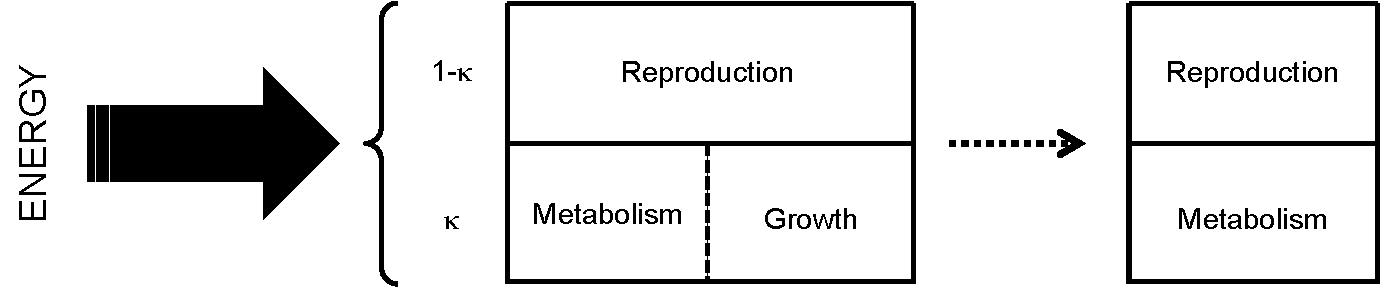
\includegraphics[width=0.95\textwidth]{4_ChapThe1/Fig/KRule}
% 
% In the $\kappa$-rule, the energy intake (thick black arrow) is first
% divided into $1-\kappa$ allocated to reproduction and $\kappa$ allocated
% to metabolism, and if all the metabolism cost is paid, the rest of
% this $\kappa$ fraction goes to growth. Once the individual has reached
% it's maximum size (dashed arrow), the energy intake is allocated to
% the metabolism and the rest to reproduction. We not that even after
% reaching its maximum size, an individual continues to reproduce until
% it cannot fulfill its metabolism anymore and dies.
% 
% Given the rules of energy allocation, we can write the individual
% growth rate and reproduction rate as functions of the functional response
% and the individual length.
% 
% Birth rate represents the production of newborns (mass or weight $w$)
% from the energy absorbed, and can be written:
% \begin{eqnarray*}
% b_{\kappa}(l) & = & (1-\kappa)\cdot\epsilon\cdot Fl^{2}\\
%  & = & r_{m}\cdot Fl^{2}
% \end{eqnarray*}
% 
% 
% where $r_{m}=(1-\kappa)\cdot\epsilon$ is a reproduction rate. We
% note that the birth rate increases with body length following a parabola. 
% 
% As opposed to reproduction which is an increase in weight, growth
% is the increase in body length $l$. We then define the parameter
% $c$ as a length to weight coefficient such as $w=c\cdot l^{3}$,
% which leads to 
% \[
% \frac{dw}{dl}=3c\cdot l^{2}\Leftrightarrow\frac{dl}{dw}=\frac{1}{3cl^{2}}
% \]
% 
% 
% Expressed in words, growth rate is the fraction $\kappa$ of the energy
% intake minus the cost of metabolism. That is to say:
% 
% \[
% g_{\kappa}(l)=\frac{dl}{dt}=\frac{dw}{dt}\cdot\frac{dl}{dw}=\frac{1}{3cl^{2}}\cdot\frac{dw}{dt}
% \]
% 
% 
% where $\frac{dw}{dt}$, the change in weight over time is 
% \[
% \frac{dw}{dt}=\kappa\cdot\epsilon\cdot Fl^{2}-\rho l^{3}
% \]
% The growth rate in body length is then 
% \begin{eqnarray*}
% g_{\kappa} & = & \frac{1}{3cl^{2}}\cdot\left(\kappa\cdot\epsilon\cdot Fl^{2}-\rho l^{3}\right)\\
%  & = & \frac{1}{3c}\cdot\left(\kappa\cdot\epsilon\cdot F-\rho l\right)\\
%  & = & \frac{\rho}{3c}\cdot\left(\frac{\kappa\epsilon}{\rho}F-l\right)
% \end{eqnarray*}
% Let's define ${\displaystyle \gamma=\frac{\rho}{3c}}$ and ${\displaystyle L_{M}=\frac{\kappa\epsilon}{\rho}}$,
% respectively the von Bertalanffy growth parameter and the absolute
% maximum length, that is to say the length at infinite resources and
% without competition, we can then write the growth rate in the case
% of the $\kappa$-rule as follows:
% 
% \[
% g_{\kappa}(l)=\gamma\cdot\left(L_{M}\cdot F-l\right)
% \]
% 
% 
% which integrates as the von Bertalanffy growth function for an isolated
% individual. We can see that with the biological interpretations of
% $\gamma$ and $L_{M}$, we don't need to have access to the value
% of $\kappa$ to parametrize the model.
% 
% 
% \subsubsection{The net production model}
% 
% 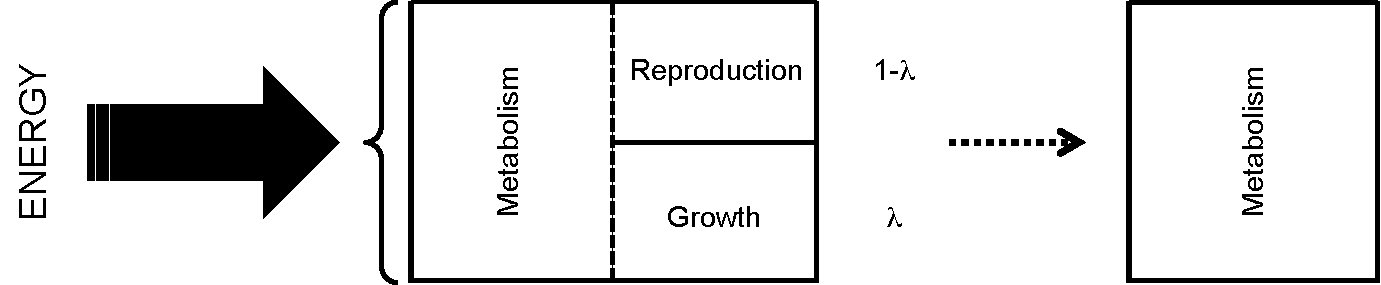
\includegraphics[width=0.95\textwidth]{4_ChapThe1/Fig/NPRule}
% 
% In the net production model, the energy intake is first allocated
% to metabolism. If some energy is left after fulfilling metabolism,
% the energy is divided between growth (fraction $\lambda$) and reproduction
% (fraction $1-\lambda$). Once the individual stops growing, meaning
% it can only fulfill its metabolism, it stops reproducing at the same
% time.
% 
% Given the rules of energy allocation, we can write the individual
% growth rate and reproduction rate as functions of the functional response
% and the individual length.
% 
% As before, the growth rate in body length can be written as follows:
% \[
% g_{\text{NP}}=\frac{1}{3cl^{2}}\cdot\frac{dw}{dt}
% \]
% 
% 
% where $\frac{dw}{dt}$, the change in wheight over time is a fraction
% $\lambda$ of what is left after paying for the metabolism: 
% \[
% \frac{dw}{dt}=\lambda\cdot\left(\epsilon\cdot Fl^{2}-\rho l^{3}\right)
% \]
% 
% 
% We can hence write the growth rate as follows:
% \begin{eqnarray*}
% g_{\text{NP}} & = & \frac{1}{3cl^{2}}\cdot\lambda\cdot\left(\epsilon\cdot Fl^{2}-\rho l^{3}\right)\\
%  & = & \lambda\cdot\frac{1}{3c}\cdot\left(\epsilon\cdot F-\rho l\right)\\
%  & = & \lambda\cdot\frac{\rho}{3c}\cdot\left(\frac{\epsilon}{\rho}F-l\right)
% \end{eqnarray*}
% 
% 
% Using ${\displaystyle \xi=\lambda\frac{\rho}{3c}}$ and ${\displaystyle L_{NP}=\frac{\epsilon}{\rho}}$
% as the von Bertalanffy growth parameter and the absolute maximum length,
% we can write the growth rate as:
% \[
% g_{\text{NP}}(l)=\xi\cdot\left(L_{NP}\cdot F-l\right)
% \]
% 
% 
% We see that $g_{\kappa}$ and $g_{\text{NP}}$ have the exact same
% form. Although the definition of the parameters differ, their biological
% interpretation remain the same, with respectively $\gamma$ and $\xi$
% the von Bertalanffy growth parameters and $L_{M}$ and $L_{NP}$ the
% absolute maximum length. 
% 
% As previously, the birth rate is the increase in mass of newborns:
% \[
% b_{\text{NP}}(l)=\frac{dw}{dt}\cdot\frac{1}{\omega}
% \]
% where $\omega$ is the weight of on newborn. With the net production
% model, the birth rate is the fraction $1-\lambda$ of the energy left
% after fulfilling metabolism:
% \begin{eqnarray*}
% b_{\text{NP}}(l) & = & \frac{1}{\omega}\cdot(1-\lambda)\cdot\left(\epsilon\cdot Fl^{2}-\rho l^{3}\right)\\
%  & = & \frac{1}{\omega}\cdot(1-\lambda)\cdot\rho l^{2}\cdot\left(\frac{\epsilon}{\rho}\cdot F-l\right)
% \end{eqnarray*}
% 
% 
% Multiplying by $\frac{\lambda}{\lambda}$ we can identify the growth
% function $g_{\text{NP}}$:
% 
% \begin{eqnarray*}
% b_{\text{NP}}(l) & = & \frac{3c}{\omega}\cdot(1-\lambda)\cdot\underbrace{\frac{\lambda}{\lambda}\cdot\frac{\rho}{3c}\cdot\left(\frac{\epsilon}{\rho}\cdot F-l\right)}\cdot l^{2}\\
%  & = & \frac{3c}{\omega}\cdot\frac{(1-\lambda)}{\lambda}\cdot\qquad\quad g_{\text{NP}}(l)\;\qquad\cdot l^{2}
% \end{eqnarray*}
% 
% 
% Furthermore, with $w=3c\cdot l^{3}$, we can write $\omega=c\cdot L_{b}^{3}$
% where $L_{b}$ is the body length at birth. We then have:
% \begin{eqnarray*}
% b_{\text{NP}}(l) & = & \frac{(1-\lambda)}{\lambda}\cdot\frac{3}{L_{b}^{3}}\cdot g_{\text{NP}}(l)\cdot l^{2}
% \end{eqnarray*}
% 
% 
% We define the parameter ${\displaystyle \beta=\frac{(1-\lambda)}{\lambda}\cdot\frac{3}{L_{b}^{3}}}$,
% and the birth rate writes as
% \[
% b_{\text{NP}}(l)=\beta\cdot g_{\text{NP}}(l)\cdot l^{2}
% \]
% 
% 
% We can see that this time that the birth rate is a third degree polynom
% which first increases with $l$, and then decreases to $0$ when the
% individuals stops growing at $l=L_{M}\cdot F$.
% 
% Going a little further, $g_{\text{NP}}$ is maximum for $l=0$ and
% $F=1$ and is equal to $g_{\text{NP}}=\xi\cdot L_{NP}$. Hence, if
% we write ${\displaystyle G(l)=\frac{g_{\text{NP}}(l)}{\xi\cdot L_{NP}}}$
% and ${\displaystyle \beta^{'}=\xi\cdot L_{NP}\cdot\beta}$, we obtain
% \[
% b_{\text{NP}}(l)=\beta^{'}\cdot G(l)\cdot l^{2}
% \]
%  where $G$ scales from $0$ to $1$.
% 
% 
% \subsubsection{From one rule to the other}
% 
% In our model, we used the $\kappa$-rule with parameters $\gamma$
% and $L_{M}$ estimated using data from experiments on the collembolan
% \textit{Folsomia candida. }The parameter $L_{b}$ is also estimated
% using the same experiments. To convert the model to a net production
% energy allocation rule, we can keep the same equation for the growth
% function, and simply estimate $\lambda$ which will give a value $\beta$,
% knowing the length at birth $L_{b}$. But $\lambda$ is very difficult
% to estimate properly. 
% 
% To decide which of the two rules are best suited to fit experimental
% or empirical data, one can look at the reproduction rate or the fecundity
% as a function of body length. A continuously growing fecundity with
% body length is an indication that the $\kappa$-rule is more fit for
% the data, wheras a bell-shaped form would tend to a net production
% model for the energy allocation. 
% 
% In the case of the collembola \textit{Folsomia candida}, measures
% on isolated individuals shows that the reproduction rate is positively
% correlated with body length, which suggests the net production model
% is not adapted and the $\kappa$-rule should be used as a dynamic
% energy budget rule for this system.
% 
% \subsection{Graphical illustration of competitive superiority of length
% $l_{\beta}$ over length $l_{\alpha}$ }
% 
% \begin{figure}[!ht] % Figure A1
% \centering
% 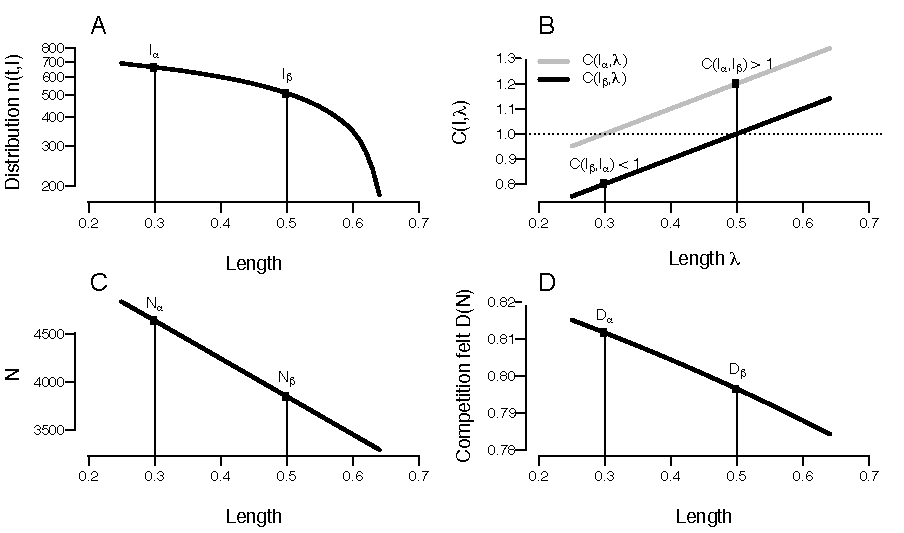
\includegraphics[width=0.85\textwidth]{4_ChapThe1/Fig/FigA1.pdf} 
% \caption{Graphical illustration of competitive superiority of $l_{\beta}$ over
% $l_{\alpha}$ when $l_{\alpha}<l_{\beta}$. A Distribution of the size giving the
% state of the population. B Competition function of individual $\alpha$ (grey)
% and $\beta$ (black) over every length present in the population for an
% interference value of $I=1$. This illustrates how much individual $\beta$ is
% competitively superior to individual $\alpha$. C Measure of the environment
% $\eta(l)$ felt by an individual of length $l$, given the state of the population
% in A. This shows that individual $\alpha$ suffers a denser environment than
% individual $\beta$. And D, resource access for the state of the population given
% in A. Individual $\alpha$ suffers a stronger competition than individual
% $\beta$.}
% \label{Fig4-A1}
% \end{figure}
% 
% \newpage
% \subsection{Fine comparison of growth rates and accessibility between $I=1.35$
% and $I=1.45$}
% 
% \begin{figure}[!ht] % Figure B1
% \centering
% 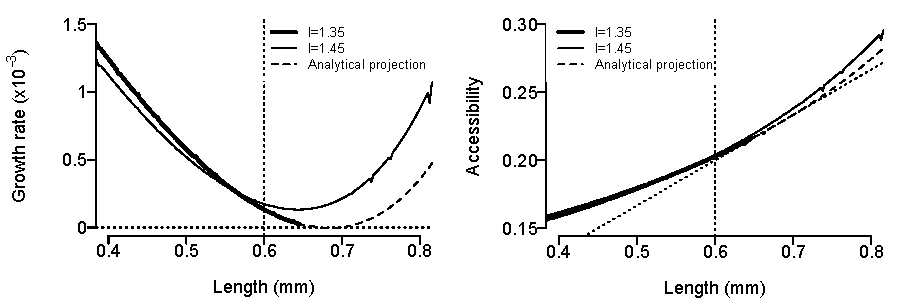
\includegraphics[width=0.85\textwidth]{4_ChapThe1/Fig/FigB1.pdf} 
% \caption{Fine comparison of growth rates and accessibility between $I=1.35$ and
% $I=1.45$.}
% \label{Fig4-B1}
% \end{figure}